\documentclass[12pt]{article}
\usepackage{fullpage}
\usepackage{graphicx}
\usepackage{amssymb}
\usepackage{epstopdf}
\usepackage{rotating}
\usepackage{multicol}
\usepackage{bbm}
%\usepackage{hyperref}
%\usepackage{cite}
\usepackage{breakcites}
\usepackage{pdfpages}
\usepackage{hyperref}
\usepackage{amsthm} % Theorem package
\usepackage{url}
 \usepackage{amsmath, amsthm}
 \usepackage{appendix}
\DeclareGraphicsRule{.tif}{png}{.png}{`convert #1 `dirname #1`/`basename #1 .tif`.png}

\title{Information Asymmetry in Profit-generating Graduate Education Markets: A Structural Approach to Law Schools
\thanks{I am indebted to my advisors, Rabah Amir and Antonio Galvao, for their direction and support. I am also grateful for helpful discussions concerning law schools with Constance Lundberg, Eric Anderson, and Reese Hansen and to Deb Tiemens for graciously allowing me access to the school-level data used in this paper. This paper benefited from helpful comments from Amil Petrin, Gautam Gowisankaran, Gene Savin, Nicholas Yannelis, Ay\c{c}a Kaya, Kyungmin Kim, Nicolas Ziebarth, David Frisvold, and Nick Street as well as comments from seminar participants at the University of Iowa, Brigham Young University, the Midwest Econometrics Group Meetings, and the SAET Conference on Current Trends in Economics. All mistakes are my own.}
}
\author{Philip J. Erickson\thanks{Department of Economics, Tippie College of Business, University of Iowa, 108 Pappajohn Business Bldg, Iowa City, IA, 52242-1994, USA. E-mail: \texttt{philip-erickson@uiowa.edu}. Website: \texttt{www.philipericksonecon.com}}}
\date{This Version: \today}                                           


% Theorem Environments
\newtheorem{theorem}{Theorem}[section]
\newtheorem{lemma}[theorem]{Lemma}
\newtheorem{proposition}[theorem]{Proposition}
\newtheorem{corollary}[theorem]{Corollary}

\theoremstyle{definition}
\newtheorem{assumption}{Assumption}[section]
\newtheorem{definition}{Definition}[section]
\newtheorem{remark}{Remark}[section]
\newtheorem{claim}{Claim}[section]

% Commands
\newcommand{\E}{\mathbb{E}}
\newcommand{\ind}{\mathbbm{1}}



\begin{document}
\hypersetup{pageanchor=false}  % turn off page numbering
\maketitle
\abstract{The number of lawyers being produced at high cost combined with the relative lack of job options has recently created significant concern. In order to partially explain this phenomenon, I propose a game of incomplete information modeling the strategic interaction between law schools as they compete for potential students. The information asymmetries come from the fact that any given law school is better informed about the quality of its education than its potential students. Using a change in market information structure generated by student placement reporting requirements, I use the model to estimate the dynamic effect of increased information on distributions of tuition rates, incoming student ability, class sizes, and the rate at which law schools open and potentially close. Using these estimates, I show that there have not necessarily been too many law schools or students, but rather an equilibrium enforced mismatch between students and their optimal schooling choices. The new information has acted as a forced collusion mechanism to partially overcome this mismatch, which has differentially decreased school welfare, strictly increased student welfare, and resulted in a positive total welfare gain of \$685 million.\medskip

JEL codes: C57, C63, C73, D22, D82, D84, D92, I23, I26, L14, L15, L52, L89

Key words and phrases: information asymmetry, higher education markets, dynamic games \bigskip \vspace{1in}
}
\thispagestyle{empty}
\newpage
\hypersetup{pageanchor=true}  % get page numbering going again
\pagestyle{plain}
\setcounter{page}{1}

\section{Introduction}
\label{sec:intro}

 Over the last decade, there has been an influx of evidence suggesting a persistent disconnect between expected and actual returns to attending law school. In 2010, the projected national market surplus for lawyers exceeded 27,000, with all but two states displaying oversupply \cite{EMSI}. Although a somewhat coarse measure, using total number of bar-exam passers (53,508 in 2009, 54,448 in 2010, and 55,387 in 2011 \cite{NCBE}) compared to projected total number of annual job openings for bar-qualified workers over the years 2010-2015 (26,239) is nevertheless telling. Further, there has been a consistent increase in both number of schools operating, with 8-20 new schools per decade and no schools closing down and enrollment increasing by roughly twenty-thousand students nationwide per decade~\cite{ABA}. Consequently, while the American Bar Association (ABA) predicts 440,000 new law graduates between 2008 and 2018, the Bureau of Labor Statistics (BLS) predicts 240,400 lawyer jobs created during that time~\cite{LSTBoverprod}.

By classical reasoning, this production behavior should be associated with an increase in the expected value of going to law school, either through a decrease in the price of attending school or through an increase in expected post-graduation earnings. Neither seems to have been the case. Nominal tuition has grown at an average rate of 6.7\% per year since 1993, 2.6 and 1.8 times more than private and public 4-year undergraduate institutions, respectively~\cite{CollegeBoard}. In 2013, the average education-based debt upon graduation from law school was over \$80,000, with 83\% of graduates from ABA-accredited schools finishing with student debt~\cite{USNews}.

Wages have not improved in real terms over this period, although they have not dropped either. Simkovic and McIntyre \cite{SimkovicMcIntyre} show stable real wages for lawyers over the past two decades, with a high mean of \$100-\$140 thousand. However, these data are for lawyers reporting to the BLS, which is not necessarily indicative of graduates from law schools in general. Besides the usual aggregate reporting bias (people happy with their salaries are more likely to report), lawyer jobs are not necessarily available to graduates of any law school. Consider, as an example, the case of Shell Oil~\cite{abovethelaw}. Shell hires in-house attorneys to handle various legal issues. Shell is certainly not one of the top lawyer positions in the country, and yet if a student graduated from a fourth-tier school, they will only consider her application at all if she was in the top 5\% of her class. This is one example of a broader phenomenon, that while students from top tier schools might be able to get a job as a lawyer, this option might not even be available to students from lower tier programs.

An answer to this apparent market failure comes in light of the information structure inherent in this market. For the majority of law students, the primary goal of attending law school seems to be to make more money (for example, in 2010 only five percent of students went in to public interest in favor of more profitable sectors~\cite{nalpSalaries}). As such, the primary school quality indicator relevant to a student should be job placement. However, until 2010, the placement number reported each year to the ABA, which governs official school-level statistics in the United States, was percentage employed nine months after graduation. This statistic does not specify if those jobs were in high paying law firms, the low skill service industry, or even at the graduate's law school with a part time position around the nine month marker. There were other secondary statistics reported, such as proportion placed in a law job or in business, but those were also fairly uninformative with respect to the quality of work.

Given this information structure, a student was left to observe job placement and impute wages from available data on lawyers, either from the BLS or from school reports to the US News. However, the BLS data are highly skewed towards graduates from top-tier programs and US News reports have suffered from underreporting and misrepresentation. A student interested in a school might think the tuition payments are reasonable given a 95\% placement rate in jobs 9 months after graduation with lawyers making \$120,000 on average per year. The danger in this reasoning was highlighted by an interview with the former Dean of the New York Law School who asserted that, while NYLS students expect to be making \$160,000 per year upon graduation, the same as graduates from Yale or Harvard, they will actually be earning a median wage of \$35-75,000 (which could be inflated as well, given that this figure was based on a 26\% reporting rate of graduates) \cite{Segal_econ}.

In 2010, in response to pressure from law school graduates and the media~\cite{Segal}, the ABA changed placement reporting standards for accredited law schools. Rather than a few vague categories, schools were now required to report a battery of specific placement types, such as ``number of students employed full time, short term in a law firm with 101-250 employees" or ``number of students employed part time short term in a state or local clerkship''. With these new reporting standards, students could look at any given school and much more accurately infer their expected post-graduation wages.

%A second major shift in the information regime, which also occurred in 2010, resulted from a crowd-sourced campaign to raise awareness of the wage disparity between law graduates conditional on quality of the law school from which they graduated. Driven initially by the New York Times' article, ``Is Law School a Losing Game?''~\cite{Segal}, the increased awareness not only caused an aggregate drop in the demand for law schools, but also made students more cognizant of the new information reporting school quality separation

In analyzing the time periods before and after the change in this market's information regime, I find significant positive and normative effects. First, using raw data and reduced form results, I show suggestive evidence that students have responded to the increased information through willingness-to-pay. Schools in lower quality brackets have had to drop tuition rates in response to a drop in the marginal valuation of their degree. Lower quality schools have also lowered their standards for admissions as measured by the LSAT scores and undergraduate GPAs of their incoming cohorts.

The relative elasticity of LSAT scores to undergraduate GPA in the incoming class combined with inelastic class sizes suggests a significant rank premium affecting a school's decision making process. To capture the rank premium, to recover student preference parameters and to allow for school shut-down and welfare calculation in counterfactual analysis, I propose a dynamic game of incomplete information modeling the interaction of schools as they compete for student enrollment.

The dynamic game and corresponding structural estimates provide values for both producer (school) and consumer (student) surplus. Schools are affected differentially by the new information policy. Top schools benefit from the quality separation as their degrees are revealed to be highly lucrative. For schools in the lower half of the top tier or in the second or third tiers, the extra information negatively affects welfare through policy adjustments tailored to maintain rank premium.

Lower third tier and fourth tier schools actually benefit from the increased information. This seemingly counterintuitive result stems from the fact that, under the previous information regime, a substantial subpopulation of lower ability potential students was being crowded out by higher ability students. 

High ability students incorrectly believed that attending a low quality law school would yield higher returns than their outside option (going straight into the labor force). These students thus were incentivized to attend low quality programs. Using the incorrect expectations, schools were able to enroll enough higher ability students to both generate a sufficient revenue stream and maintain their relative standing among other schools. This behavior by schools resulted in excluding lower ability students from enrollment, who, based on their outside option, would have actually benefited from a low quality law degree.
%degree from a low quality program.

The new information regime acts as an exogenously imposed collusion mechanism. All lower quality schools are forced to simultaneously reveal that their product is of lower value than many of their previous students' outside options. Since all schools act simultaneously, there is little rank effect since ranks are relative. Further, all low quality schools now have access to the previously underserved subpopulation of lower ability students, thus actually increasing enrollment and consequent tuition revenue.

%Any given low quality school, privately understanding the benefit of their degree to lower ability students, could have dropped its admissions standards and also accepted students from this underserved population. While admitting these students would have increased immediate tuition revenue, the corresponding drop in rank would have damaged the school's future returns enough to make this behavior suboptimal. Thus, the previous information structure maintained an equilibrium-enforced systemic mismatch between schools and students.

%The new information regime acts as an exogenously imposed collusion mechanism. All lower quality schools are forced to simultaneously reveal that their product is of lower value than many of their previous students' outside options. Since all schools act simultaneously, there is little rank effect since ranks are relative. Further, all low quality schools now have access to the previously underserved population of lower ability students who, based on their outside options, still face positive returns to attending these programs. 



%potential students consists of lower quality candidates who would be happy attending lower quality schools, even after the change in reporting standards, but were previously unable to do so as they were crowded out by higher ability students who, under the previous information regime, incorrectly believed that attending a lower quality school would provide higher returns than their outside option (going straight into the labor force).

% inefficiently attending lower quality schools. The low ability students were in essence barred from participation by a systemic mismatch between students and schools in the lower quality brackets.

%A low 

%Unilateral deviation 

%While unilateral deviation from the mismatch by any given school was suboptimal given the ensuing drop in profits through the rank premium, the extra information acted as an exogenously imposed collusion mechanism, resulting in all schools of a certain bracket simultaneously lowering their admissions criteria, both enrolling more students from the underserved population and not losing money through the rank premium (since ranks are relative).

%The schools in the bottom half of the bottom bracket are revealed to have a product of such low quality as to not gain from the expansionary effects enjoyed by low to middle quality schools.

The aggregate change in producer surplus is negative with a mean estimate of -\$212 million. Much of the loss to producer surplus is recovered by students as they receive a product, either through going to law school or opting out of the market, consistent with their preferences and abilities. The aggregate consumer surplus change is \$575 million, resulting in a total surplus gain of \$363 million.

The idea that students have incorrect expectations concerning returns to schooling has been the subject of several previous studies. Manski \cite{Manski04} discusses this phenomenon, explaining how students often can have post-education wage expectations different from reality. Arcidiacono, Hotz, and Kang \cite{ArcHotzKang} estimate expectations of the return to choosing a particular major. They show that, not only do expected earnings matter when students choose a major, but students' expectations with respect to major-specific earnings are often wrong. This inconsistency between schooling expectations and reality can partially explain why students are willing to pay for a degree in a low-return field, with schools using these expectations to extract tuition rent.

The problem of using information frictions between students and schools to inflate profits is indicative of a broader phenomenon. That is, information asymmetry with respect to product differentiation can have serious effects on proper function of market. In the case of law schools, schools have had more information that students concerning the quality of their product (law degree). Dranove, et. al.~\cite{DranoveEtAl} show in the market for health care that when patients are better informed concerning the quality of any specific hospital, prices and general treatment both improve while hospitals also change the type of risk they are willing to take on. This change in healthcare behavior gives evidence that hospitals can use information asymmetry to affect prices in a similar way to law schools. Jin and Sorenson~\cite{JinSorenson} show that consumers choose health plans consistent with published information available, but inconsistent with some important unpublished indicators of quality. Health plan providers can extract rent based on the information asymmetry between themselves and their clients.

While previous work has shown how information can affect prices and demand for a product, this is the first paper, to my knowledge, to document a systemic mismatch between consumers and producers created by information frictions. This mismatch is due in large part to the two-sided nature of the legal (or any) education market in which the quality of the consumer also matters to the producer. The paper also gives encouraging evidence that information availability can provide a market-based approach to at least partially mitigating this mismatch.

% --------------------------- %
%    INFORMATION STRUCTURE    %
% --------------------------- %
\section{Information Structure}
\label{sec:infostructure}
%This awareness campaign began as a series of blog posts from law school graduates facing difficulty paying off their student debt, but 
Information in the market for training lawyers is largely governed by the ABA. The primary function of the ABA is to set accreditation standards for law schools in the United States. If a school is not ABA accredited, its students may not (with the exception of California) take the bar exam. Thus, for a school to be viable, it must be ABA accredited. One of the primary tools the ABA uses to make accreditation decisions is its yearly school questionnaire, which is published each year jointly with the Law School Admissions Council (LSAC) as part of the ``ABA-LSAC Official Guide to ABA-Approved Law Schools''~\cite{LSAC}. This questionnaire provides statistics on various attributes of a school such as Curriculum, JD Enrollment and Ethnicity, GPA and LSAT Scores, and Grants and Scholarships. For a sample of a pre-2010 questionnaire, see Appendix~\ref{app:questionnaires}.

Much of the information reported in the ABA-LSAC report might be interesting or important for reasons pertaining to social issues (ethnicity and gender of students) or to educational atmosphere (student to teacher ratio or number of professional librarians). However, based on the prevailing motivation to attend law school, the indicator of most concern to a student deciding which, if any, school to attend should be expected wages after graduation.

In reports issued before 2010, placement success was primarily measured by the number of students placed in a job nine months after graduation. There were also refinements given, including number employed in law firms, in business and industry, in government, in public interest, as judicial clerks, or in academia. However, these refinements gave little information with respect to salaries. A student employed in a law firm could make anywhere from \$30-130 thousand a year. An employee in ``business'' could likewise be earning a high salary on a management track at a large corporation or minimum wage working in a low-skill sector.

Since the traditional ABA-LSAC report was mostly uninformative concerning post-graduation wages, if a potential student wanted to go to law school, she would have to make a judgement based on the data provided for the market for lawyers in general and extrapolate from the data provided by a law school for the ABA-LSAC report. She might see, for example, a low-ranked school that places 85\% of its students in a job nine months after graduation, see BLS report that lawyers make \$120,000 per year and reason that it would be a good investment to take on \$100,000 in student debt to get that degree.

This extrapolation does not, however, fit the reality of the lawyer market. Oyer and Schaefer show that, not only do graduates from the top 20 law schools comprise the majority of partners and associates in the top major law firms in the United States~\cite{OyerSchaefer10}, but graduates from the top 10 schools make 25\% more money than those from top 11-20 schools and 50\% more than those from schools ranked from 21-100~\cite{OyerSchaefer09}.

An alternative to the BLS wage reports is the Starting Salaries~\cite{nalpSalaries} report from the National Association for Law Placement (NALP). This report has been produced in an attempt to decrease the information gap between student expectation and reality by reporting wage statistics for each of the reported categories in the ABA-LSAC report. However, since the NALP does not have the same influence as the ABA, it has not been able to maintain substantial reporting rates. For example, while over 40,000 lawyers passed the bar exam in 2010, there were only 18,398 respondents in total who responded to the NALP survey. Further, those reporting are generally also those making more money~\cite{Segal_econ}.

While schools have generally been aware of the disparity between students' wage expectations based on available data and the realities of the market~\cite{Segal_econ}, they have been able to use their asymmetrically high information set to extract rent from ever more students in the form of tuition revenues as new schools have opened, class sizes have grown, and tuition rates have increased.

In an attempt to mitigate this issue, in 2010 the ABA modified its reporting requirements. Rather than fifteen vague categories, schools were now required to report on 144 specific placement types. Rather than ``Employed,'' a school would now have to report various types of employment, such as ``Employed - Bar Passage Required, Full Time, Short Term.'' Rather than ``Employed in a Law Firm,'' a school would now have to report on the size of the firm, such as Solo, 2-10, 11-25, 251-500, etc. The firm size reports are especially informative given information made available by the NALP. Besides average starting salaries in general industries, the NALP also reports starting salaries at law firms conditional on firm size. Table~\ref{tab:nalp} is an example report from 2011~\cite{NALP2011}.
\begin{table}[htp]
\begin{center}
\begin{tabular}{lcccccc}
\hline
\hline
Firm Size & 2-10 & 11-25 & 26-50 & 51-100 & 101-250 & 251 or More \\
Salary & 73,000 & 73,000 & 86,00 & 91,000 & 110,000 & 130,000 \\
\hline
\end{tabular}
\end{center}
\caption{Median Lawyer Starting Salary per Firm Size (2011)}
\label{tab:nalp}
\end{table}
As stated before, these numbers are likely biased. However, given the motivation behind the reporting bias is aversion to reporting and getting reports on low salaries, the bias should either be uniform across category types or more severe for lower-sized firms, generating lower wages generally. The difference in reported wages between small firms and large firms should therefore be a lower bound on the actual spread. The lower bound is still substantial, with the difference in earnings expectations between the largest and smallest firms reaching almost \$60,000. Because of the reporting change, students debating law school attendance post-2010 can use the newly reported categories combined with these wage reports to make a better informed decision about which, if any, law school to attend.

Besides the ABA and the NALP, the US News and World Report provides one more major source of information. Although the US News does not provide a large number of school characteristics for public consumption, it does serve as the primary data aggregator in this market through its primary instrument, the US News and World Report Graduate School Rankings~\cite{USNews}.

To construct its rankings for law schools, the US News utilizes data required for the ABA-LSAC report as well as several of its own measures. The most notable variables with regard to salary expectations are percentiles for starting salaries of law school graduates. While these measures should be the most informative to students, they have traditionally possibly exacerbated the information asymmetries due to low reporting standards, with documented evidence of schools reporting their graduates earning as much as \$100 thousand more on average than they actually were~\cite{Segal_econ}.

% ---------- %
%    DATA    %
% ---------- %
\section{Data}
\label{sec:data}
The market for training lawyers is characterized by two general sets of players: schools and students. To estimate parameters relavent to both sets, I utilize both school-level and student-level data. For initial results showing effects in the market in Section~\ref{sec:rf}, I will only use school-level data. Individual-level data will be necessary for identifying welfare effects in Section~\ref{sec:structural}.

\subsection{School Level}
\label{sec:data_school}
School-level data were taken from the start of academic years 1998-2013, which are designated as the years 2000-2015 for both the ABA-LSAC report and the US News and World Report rankings data. The US News data includes both the rankings and extra data used to for the rankings not included in the ABA-LSAC report. Summary statistics are reported in Table~\ref{tab:summary}. 

The variables reported represent student quality and school characteristics.  Quality is given by two measures. The measure is the US News Rank. While US News rankings certainly do not give a perfect quality separation measure between schools, it does give a reasonable approximation of tiers. For example, \#1 ranked Harvard clearly has a better law program than the \#144 ranked South Texas College of Law.

The second quality variable not only measures quality separation, but also explicitly captures the new information made available to students concerning school quality. I define this measure as a school's \emph{placement ratio} which is constructed using the new information available with the post-2010 ABA/LSAC reports.

I first take a weighted sum of graduate placement in law firms, weighted by firms size according to the 2011 NALP report in Table~\ref{tab:nalp}. I normalize the highest possible wage to unity, representing a ``full" placement. Each subsequent category is weighted as the fraction of the highest possible wage. For example, each placement in a firm with 51-100 employees would be weighted by (91,000 / 130,000), or 0.7. For solo firms, I assume the same wages as the next two smallest firm categories. I put zero weight on placements in firms of unknown size.

After generating the weighted placement, I divide it by raw placement numbers in law firms. Since I normalize the highest possible wage to unity, this ratio will always lie strictly on the unit interval. As is shown in Table~\ref{tab:summary}, the mean and median are close at 0.64, indicating that the average school is placing its students at jobs with starting salaries only 60\% of the top salaries. The best placing school is gaining its graduates 97\% of the top salaries on average and the worst placing schools are achieving 33\%.

For the placement ratio to be useful, it must span all the time periods available in the data. However, by definition, it cannot be calculated earlier than 2010. I use ratio persistence to motivate an imputation solution. A basic AR(1) model yields an AR coefficient of 0.915 with a standard error of 0.015. Thus, I impute the ratio for all previous years as that calculated for 2011 and designate this variable as each school's persistent type.

Tuition is the price of attending law school while Freshmen is the size of the incoming class. This class is characterized by its average undergraduate GPA and LSAT scores. Schools also award grants and have other room/board expenses, cost of books, large or small faculties relative to student body size, acceptance statistics, and Bar examination passage rates at first attempt.

The variable for tuition is constructed from the sticker price for a full-time out-of-state student for schools that price discriminate based on residency and standard full-time tuition for schools that do not. I discuss the use of sticker price more in depth in Section~\ref{sec:structural}. Since the tuition reported in any given ABA-LSAC report actually corresponds to the tuition paid by the previous year's students, I lag tuition by one year. The lag aligns payments with the academic year represented by the rest of the report.

Table~\ref{tab:summary} also shows summary statistics for 25th and 75th percentiles of reported private sector salaries. The mean 25-75th percentile spread is about \$56-89,000 which is somewhat higher than the median spread of \$48-80,000. These suggest a possible median salary in the range of \$64-72,000, which is about \$10-20,000 lower than the salaries implied by the transparency ratio. And once again, although better than the NALP, reporting rates are somewhat low, with mean and median rates of 61\% and 64\%, respectively. Since schools are aware that students are highly influenced by the rankings developed by this report, the salary reports are once again likely biased upwards.

\subsection{Student Level}
\label{sec:data_student}

Student-level data were taken from Law School Numbers (LSN)~\cite{lsn}, an online resource for potential law students. LSN was created primarily as a forum for law school applicants to report on application, admission, and enrollment decisions as they go through the process of possibly attending law school. LSN makes these reports publicly available as a crowd-sourced database on the state of law school applications and admissions.

A unit of observation in the dataset extracted from the LSN reports is a school-student pair, with one observation for each pair. Each observation includes the year of the potential match, the student's profile, consisting of her LSAT score and undergraduate GPA\footnote{GPA is reported for both raw degree GPA, the number reported on the student's diploma, and the LSAC-adjusted GPA, which is the one used by law schools for admission decisions.}, the name of each school she applied to, and the result of that application, including whether or not the student was accepted (or waitlisted) and the student's decision (whether or not she decided to matriculate).

Various summary statistics for the LSN dataset are reported in Tables~\ref{tab:summary_appadmit}, \ref{tab:summary_quant_GPA}, and \ref{tab:summary_quant_LSAT}. Table~\ref{tab:summary_appadmit} provides student summaries conditional on one of three stages of the school admissions process: application, admission, and matriculation. Tables~\ref{tab:summary_quant_GPA} and~\ref{tab:summary_quant_LSAT} summarize the entire student sample by ability quartile. In all tables, statistics are provided for student samples under the old and new information regimes.

From Table~\ref{tab:summary_appadmit}, it seems that the applicant skill distribution remains practically unchanged under the new information regime. The biggest difference between the two samples is in admission and matriculation probabilities. In the treatment period, probability of admission increases by roughly 0.06 while probability of matriculation decreases by 0.06 percent. Although small, this is indicative of a phenomenon that will be studied more in depth later in the paper. Specifically, schools face smaller applicant pools under the new information regime and students have a lower valuation of certain types of law degrees, thus decreasing matriculation probability.

The information effect is further emphasized in Tables~\ref{tab:summary_quant_GPA} and~\ref{tab:summary_quant_LSAT}. While once again, the distribution of applicant type remains virtually unchanged across information regimes, admission and matriculation probabilities change again, with most of the difference observed in the second quartile of students. Once again, this difference indicates a decrease in options for middle to high quality schools as well as a shift in expectations for middle to high ability students.


% Discuss this?? While participation in this dataset is purely elective, the distribution of 

% ------------------ %
%    REDUCED FORM    %
% ------------------ %
\section{Evidence of Information Effects}
\label{sec:rf}

Behavior of law schools with respect to students has evolved according to the information structure as well as market indicators. Figures~\ref{fig:rank_quantile} and~\ref{fig:ratio_quantile} provide visualization of the primary variables of interest. These variables include tuition rates, number of students, incoming class profiles (undergraduate GPA and LSAT scores), number of applicants, grant awards (both number and size), and starting salaries of graduates (25th and 75th percentiles).

\subsection{Conditional Quartiles}

Each variable is divided into quartiles based on school quality. In Figure~\ref{fig:rank_quantile}, quality of a given school is measured by its rank as assigned by the US News and World report. As previously discussed, this is a standard quality measure in this market. In Figure~\ref{fig:ratio_quantile}, I use the placement ratio as defined in Section~\ref{sec:data_school}.

Since the placement ratio was not observed before 2010, behavior of students and schools conditional on the ratio should change based on being in a post-2010 world. The population thus becomes a policy treatment group with treatment being the new school-idiosyncratic information administered starting in 2010. Ideally, the data would include a control group as well, unaffected by this extra influx of information. Although there is no strict control group, I can utilize the fact that the top schools would be expected to place almost all their students in the most competitive jobs. Thus, the extra information would technically have a negligible effect on these programs. These schools could thus be considered a quasi-control group and the treatment could be considered as given post-2010 in some varying amount over the compact interval [0, 1], with 0 indicating a full dose and 1 indicating no treatment.

US News ranking as a quality measure does not \emph{explicitly} capture the information effect of 2010. \emph{Implicitly}, the same school behavior stemming from the extra information in 2010 should be observed with respect to rank as well since rank and placement ratio are highly correlated, with a correlation coefficient of -0.75 for the years in which placement ratio can be directly observed.

\subsection{Variable Evolution}

There are two main features of Figures~\ref{fig:rank_quantile} and~\ref{fig:ratio_quantile}. The first and most obvious is the aggregate drop in the market in 2010. This drop stems from two sources. The first is the great recession of 2008. While many industries were effected immediately by the market downturn, the effect on the market for lawyers lagged roughly two years behind the rest of the economy. This effect is born out primarily in legal salaries, as can been observed primarily in the 75th percentile of salaries and somewhat in the 25th percentile as well.

While the effects of the recession could have a trickle down effect on school and student behavior, such as application rates and quality of students going to law school, it is likely that this is not the primary driver behind the corresponding aggregate shocks in these other variables. This is due to the fact that the recession-based shock affected all industries, not just lawyers. Without a stable outside option, substitution effects should be small.

The second source of this aggregate drop in the market, however, was idiosyncratic to the market for lawyers. Between 2010-2011, the legal market experienced an aggregate opinion shift regarding law degree profitability. Stemming from the seminal New York Times article by David Segal, ``Is Law School a Losing Game?''~\cite{Segal}, a sentiment developed in the United States that many students were graduating from law school, apparently without a way to pay back loans incurred during schooling. Segal, and many authors following him, contended that going to law school might not in fact be profitable on average. The ensuing series of articles, blog posts, etc. sparked an aggregate downturn in demand for law school. This is likely one of the primary causes of the drop in applications to law school beginning in 2010.

The second feature of note in Figures~\ref{fig:rank_quantile} and~\ref{fig:ratio_quantile} beyond the aggregate shocks is the separation in several variables between quantiles after 2010. The most obvious is undergraduate GPA of a given school. In both Figure~\ref{fig:rank_quantile} and Figure~\ref{fig:ratio_quantile}, the lower the quality of school, the more it had to drop its threshold for the quality of student it would admit. The same separation holds for Tuition as well, although more prominently in Figure~\ref{fig:ratio_quantile}.

While it is clear that the separation holds for GPA, it seems possible upon visual inspection that it might also be occurring in the other variables. This could be of concern when trying to identify the effects of information. Specifically, if there is a significant separation of salaries conditional on quality after 2010, it could be that the recession effects are primarily driving the altered school behavior. The same holds for the aggregate dropped expectations of the return to law degrees and number of applicants to law school.

To test for the presence of quality conditional post-2010 separation, I propose the following specification
\begin{equation}
	y_{it} = \beta_0 + \beta_1 R_{it} + \beta_2 Post2010_t +
			 \beta_3 (R_{it} * Post2010_t) + \gamma X_{it} + \varepsilon_{it},
	\label{eq:diff_in_diff}
\end{equation}
with $R$ either rank or ratio and $y_{it}$ either one of the primary school outcome/choice variables including class size and tuition (quantity and price) and quality of students willing to attend (GPA and LSAT scores) or one of the other market variables (starting salaries or number of applicants). $X$ is a vector of controls from the set \{\{Rank\}, \{Tuition, Median Undergraduate GPA, Median LSAT\}, \{Median Grant, Percent Receiving Grants, Room/Board Expenses, Cost of Books\}, \{Student/Faculty Ratio, Number Accepted, Acceptance Rate, Bar Passage Rate in Jurisdiction\}\}. Note the subsetting of $X$. These subsets correspond to models controlling for 1) rank (in the case of $R=$ ratio), 2) school choice variables, 3) cost variables, 4) miscellaneous quality controls. Each model will be estimated separately as well as once with all four sets of controls.

For each possibility for $y$, $\beta_3$ is the primary parameter of interest. Since an increasing value of ratio and a decreasing value of rank both indicate an increase in quality, the sign of $\beta_3$ should be opposite between the two. I will proceed discussing the case of $ratio$, but with the understanding that the converse should also hold for $rank$.

I first address the question of either application or salary separation to determine if they might confound identification of the desired information effect. Consider first the model with $y=$ number of applications. The results are given in Tables~\ref{tab:apps-ratio} and~\ref{tab:apps-rank}. Notice that most of the model specifications result in an estimate of $\beta$ statistically indistinguishable from zero. The exceptions in both cases are when admission rates are included as controls. However, this could yield artificially significant results because of the high collinearity between number of applications and application rates.

The more worrisome results are in Tables~\ref{tab:sal25-ratio}, \ref{tab:sal25-rank}, \ref{tab:sal75-ratio}, and \ref{tab:sal75-rank} which correspond to 25th and 75th percentile salaries. With $R=$ ratio, $\beta_3$ is significant and positive for both percentiles under every model specification. However, for $R=$ rank, the significance almost completely disappears. If both the ratio and rank specifications had yielded a significant interaction coefficient, there could have been strong evidence that salaries themselves are driving the separation in the other variables. However, the disparity between the two sets of models suggests that the connection between the ratio models and salary separation is part of some process outside of the effect connecting ratio and rank. As long as both the ratio and rank models yield the correct values for $\beta_3$, this would provide evidence that the information effect is indeed being identified. 

If the information treatment is effective, $\beta_3$ should be positive for ($y=$ Tuition). That is, $\beta_3$ represents the immediate shift in students marginal valuation of a degree from any given law school based on increased transparency due to information restructuring.

For GPA, LSAT and Class size, $\beta_3$ depends on a school's dynamic consideration. A school with a decreased reputation could maintain class size and drop the quality of students it accepts. This way, it can maintain immediate revenue. However, lowering student quality also hurts its future rank, which decreases its future revenue. The elasticity of GPA, LSAT, and Class size will depend on how much a school could gain or be hurt in the long or short run. The estimates for Model~\eqref{eq:diff_in_diff} for dependent variables Tuition, Class Size, Undergraduate GPA, and LSAT are given in Tables~\ref{tab:tuition-ratio}~\ref{tab:class-ratio}~\ref{tab:gpa-ratio} and~\ref{tab:lsat-ratio}.

As expected, Tuition responded significantly to the information shock. For the baseline estimate with no controls, the treatment coefficient indicates that a school with a 10 percentage point higher placement ratio will have a \$1.6 thousand higher marginal valuation on the part of its students. This increases when controlling for Rank to \$2.7 thousand, but drops to between \$600 and \$1.2 thousand for other control specifications.

Controls are based on incoming class profile (Freshman Class Size, Undergraduate GPA, and LSAT scores), cost structure (Median Grant, Percent Receiving Grants, Room/Board Expenses, and Cost of Books), and other quality controls (Student/Faculty Ratio, Number of Students Accepted, Acceptance Rate, and Bar Passage Rate in Jurisdiction). Incoming class profile seems to account for much of the extra variation in tuition rates (highest effect on $R^2$), as well as part of the covariance between the treatment effect and Tuition.

The model only controlling for freshman profiles is the only model that causes the significance of the treatment effect to fall below the 0.001 level. However, the significance jumps back when including the other controls as well.

In the final estimate, most of the variables are highly significant. The three exceptions are Post-2010, the level-effect for being in treatment period; Freshmen, the size of incoming class; and Bar Passage Rate. Class size is likely highly correlated with some of the other controls, making its insignificance in the full model not surprising. Bar Passage Rate was never significant, which is surprising. Post-2010 is not only most insignificant across specifications, but also changes signs frequently.

The treatment level effect is likely insignificant for two connected reasons. First, the other variables in the dataset account for much of the variation in Tuition. Second, the treatment period is relatively short. This makes the fact that the treatment effect is so significant even more surprising. In the final model with all controls included, $\beta_3=9112.45$, suggesting that a school with a 10 percentage point higher placement ratio would optimally be able to charge \$911.25 higher price for its product.

The coefficient estimates for the class size and student profile models shed light on the profit structure for law schools. First, as is seen in Table~\ref{tab:class-ratio}, class size seems to be completely inelastic with respect to the information shock. The ratio-treatment interaction coefficient is insignificant in every model specification. LSAT scores are similarly rigid. While the coefficients are all technically positive, none are significant.

Schools are statistically more flexible with the undergraduate GPA scores of incoming classes, although the substantive reaction is small. For the baseline specification with no controls, the ratio-treatment coefficient is $0.17$. This coefficient implies that a school that dropped 50\% in its expected returns would have to lower its GPA standards by roughly 0.09 GPA points. The change could also be as small as 0.045 GPA points. Across every specification, though, this change is significant and is on average about 0.07.

Few of the controls are significant predictors of GPA and are motivated, not by causation, but because of joint indication of school or student quality. For example, students with higher GPAs will likely have higher LSAT scores. Thus, the LSAT coefficient is significant. GPA is also understandably negatively correlated with acceptance rate, since in order to increase the student quality threshold, a school must be more selective in accepting students.

\subsection{Discussion}

The relative elasticity of tuition compared to class size is indicative of inelastic supply with respect to demand. The change in information in 2010 would represent a demand shift for any given school. As is well known, if the supply is relatively inelastic with respect to demand, we would expect to see a large change in market price but little to no change in the quantity being produced.

Inelasticity of supply indicates a high marginal cost of producing students. In the case of law schools, this would arise not in direct marginal cost, but in the forgone rank premium associated with enrolling a higher number of students. As a school admits the marginal student, it must lower its quality threshold to allow a marginally less qualified student to attend. In doing so, although the school gains in current tuition, it loses future profits related to the drop in prestige.

The argument of a high rank premium is further born out in the relative flexibility of GPA compared to LSAT scores. LSAT scores are not only considered a more important prestige measure for a school, but they are also weighted 40\% more in the US News ranking formula. Given that schools apparently find it optimal to maintain class size, they would rather lower GPA standards than the more valuable LSAT standards.

% ------------- %
%     MODEL     %
% ------------- % 
\section{Structural Framework}
\label{sec:structural}

The reduced-form evidence in Section~\ref{sec:rf} suggest that the new information regime has changed the way that students view any given school as well as how schools can behave with respect to students. It also highlighted that schools seem to make dynamic decisions with respect to payoff-relevant variables like class size and quality. However, the discussion thus far has been agnostic concerning the normative effects of the new information regime. The question remains, has this influx of information been good for the economy? If so, in what way and for whom? To determine societal welfare effects, it is necessary to impose additional structure.

As stated, the reduced-form evidence suggests a dynamic decision-making process. A school's dynamic considerations should be with respect to its own evolution as well as to the evolution of its competitors. Each time a school tries to attract students, it is competing for those matriculations with several other schools of similar quality. As such, to model the dynamic considerations of a school, it is necessary to include the strategic effect.

Modeling this market as a dynamic game also has the benefit of allowing identification and estimation of structural payoff-relevant parameters otherwise unattainable. As was discussed in the previous section, the behavior of schools suggests a high rank premium. This should affect schools not only though tuition revenue, but also through donations and grants, a significant source of revenue but unobservable in the data. The structure imposed in the following section will allow for identification of parameters associated with the rank premium and allow for calculation of producer (school) surplus. The extra structure will also provide identification for the utility for individual students from attending law school as well as their outside option. Thus, we can also analyze consumer (student) surplus.

Structural estimates are also necessary for positive dynamic analysis concerning entry and exit of schools. As stated earlier, between 8-15 new law schools have opened nationally per decade for many years. There has, however, been no exit. The estimates of Section~\ref{sec:rf} suggest that profitability for schools, especially low quality schools, could decrease. For some schools who entered the market with the expectations of high revenue payments, the profitability drop could lead to shut-down.

In order to capture all the relevant player characteristics, I propose a school choice model based on the application/admission game in Fu~\cite{Fu}, but extended to a dynamic framework in the tradition of Maskin and Tirole~\cite{MaskinTirole} and Ericson and Pakes~\cite{EricsonPakes}. The dynamic extension allows for explicit consideration of rank effects as well as entry/exit decisions. In this setting, time is infinite and discrete and players discount future returns at rate $\beta$.

\subsection{Players}
\label{sec:players}

The market for training lawyers is characterized by two sids of players: schools and students. Schools act as competing oligopolistic firms producing their good, a law degree, for their consumers, prospective students.

Schools, each consisting of a tuition office and an admissions office, are differentiated by their rank which acts as a proxy for relative quality. In this application, rank will be operationalized by a school's rank as measured by the US News and World Report \cite{USNews}. A more in-depth discussion of the use of US News rankings was given in Section~\ref{sec:data}. A rank of zero indicates that the school is not operating (that is, it has not yet opened or has closed). In any period, the state is represented by the tuple $(R, g)$. $R$ is a vector of length $\overline{N}$, where $\overline{N}$ is the maximum possible number of operating schools and $R_j\in R$ is the rank of school $j$ in the current period for any $j\in J$, the set of currently operating schools. The remaining state variable $g$ is a demand growth term that will be discussed later. Each school is endowed with a fixed capacity $\overline{Q}_j$ with $\overline{Q}_j > 0$ and $\sum_{j=1}^{\overline{N}}\overline{Q}_j < 1$.

The rank vector is proxy for the production technology available to any given school. That is, a school ranks represents what quality of a product the school can produce. In the case of law schools, quality of a program is assumed to be the expected financial returns to getting a degree. Although some students do enter law school on more philanthropic grounds, given that only five percent of 2010 law graduates went in to public interest in favor of more profitable sectors \cite{nalpSalaries}, the assumption that students attend law school in order to purchase a better wage distribution seems reasonable.

The other state tuple element, $g$, is a time-specific demand shifter. This will grow according to a degenerate process and captures the persistent exogenous effects on aggregate tuition growth in law schools. This is in large part due to an increase in federal funding and loans to law students and is connected with the perceived benefits of attending law school in general~\cite{nyt_debt_crisis}.

There is a continuum of students, normalized to unit measure. Students differ in ability endowment $A$, which is unobserved but correlated with a student's LSAT score and undergraduate GPA, given by the tuple $(LSAT, GPA)$. I assume A is distributed $N(f_A(LSAT, GPA), \sigma_A^2)$, with $\partial f_A / \partial LSLAT > 0$, $\partial f_A / \partial GPA > 0$, and $\partial^2 A / \partial LSAT \partial GPA > 0$.

In order for student $i$ to apply to school $j$, she must pay the application cost $C(\cdot)$, which is increasing in number of applications.

\subsection{Stage Game}
\label{sec:stage_game}

In each period, students and schools play an application/admission game in the spirit of Fu~\cite{Fu}. The timing of the stage game is as follows: first, each school announces a tuition level to which it must commit (which gives the game a Bertrand-type competition structure, since tuition represents the price in this market); second, students make application decisions while schools simultaneously choose admission policies; and third, students learn about admissions results and make enrollment decisions.

\subsubsection{Student Payoffs}
\label{sec:student_payoffs}

The preferences of student $i$ with ability $A$ with respect to attending school $j$ of rank $R$ is given by the random indirect utility function
\begin{equation}
  u_{ij} = \overline{u}(A_i, R_j, I) + \epsilon_{ij}
  \label{eq:student_preference}
\end{equation}
with $\overline{u}(\cdot)$ the average preference for a student with ability $A$ to attend a school with rank $R$ and $\epsilon_{ij}\sim N(0, \sigma^2_u)$ student $i$'s idiosyncratic preference for school $j$. The realization of $\epsilon$ occurs after admissions decisions have been made. The variable $I$ is binary and represents the information regime in place, with $I=0, 1$ indicating the previous and current regimes, respectively.

I assume that all students pay the same sticker price tuition rate, or that there is no price discrimination in this market. This assumption ignores scholarship behavior, an important aspect of the market, and is made due to data limitations\footnote{See \cite{Fu} and \cite{Fillmore} for examples in which price discrimination is explicitly modeled.}. However, since the primary goal of the analysis at hand is to study the welfare changes from the introduction of a new information regime, the only cause of potential bias would come from a systematic change in price discrimination behavior based on the regime change. While the data in Figure~\ref{fig:rank_quantile} suggest that there is unlikely to be such a change, potential biases from this omission will nevertheless be discussed in Section~\ref{sec:structural_est}.

For tuition profile $t\equiv\{t_j\}_{j\in J}$, the ex-post payoff to student $i$ for attending school $j$ is
\begin{equation}
  U_{ij}(t) = u_{ij} - t_j.
\end{equation}


%There is also a substantial amount of price discrimination beyond the sticker price of a degree from any given institution, which can be identified given the appropriate amount of student-level data \cite{Fillmore}. However, as long as price discrimination behavior is consistent across school types, it is admissible to focus on the sticker price. This seems reasonable in light of Figure~\ref{fig:rank_quantile}. If sticker price is higher or lower relative to average price for higher quality schools than lower quality schools, then the rank-coefficients for the equilibrium tuition reaction functions would be biased high or low, respectively. Otherwise, the rest of the analysis would remain the same.

\subsubsection{School Payoffs}
\label{sec:school_payoffs}

Period profits for an individual school are derived from tuition revenue as well as yearly donations and fixed costs. Tuition revenue is given by
\begin{equation}
  \tilde{\pi}_j = \int t_j dF_j(i)
  \label{eq:tuition_rev}
\end{equation}
with $F$ defined as the endogenous distribution of admitted students.

Revenue Donations come mostly in the form of alumni giving as well as earnings from private and public endowments/grants and are a function of the school's rank. While there are effectively zero explicit marginal costs for schools (although there are implicit marginal costs through reputation effects, which are discussed below), fixed costs are substantial and vary according to quality of a school. Higher quality schools generally offer higher faculty salaries, have better and more expensive resources that require maintenance and replacement, etc.

Although donations and fixed operation costs are not separately identifiable, since they are both functions of rank I can identify donations net of operating costs with a net donation function. I parameterize the net donations with the quadratic function
\begin{equation}
  D(R_j; \delta) = \delta_1 R_j + \delta_2 R_j^2.
  \label{eq:donations}
\end{equation}
If fixed costs are greater then than yearly donations, $D$ will be negative. There is possibly also some fixed cost $\delta_0$ associated with running a school regardless of rank. I exclude $\delta_0$ from the model since, because I do not observe cases in which schools shut down but do not leave the market, I cannot identify it in the data. However, as long as $\delta_0$ is independent of the information regime, its exclusion will not bias the final results with respect to change in welfare.

An inactive school deciding to open draws a fixed entrance cost $\kappa$ at the beginning a period from the distribution $N(\mu_\kappa, \sigma^2_\kappa)$. Incumbent schools also at the beginning of a period receive a scrap value draw $\phi$ from distribution $N(\mu_\phi, \sigma^2_\phi)$. Thus, a school $i$ participating in action $a$ receives the period profit adjustment
\begin{equation}
  \Phi(a_j; \kappa_j, \phi_j) =
  \begin{cases}
    -\kappa_j, & \text{ if the school is a new entrant} \\
    \phi_j, & \text{ if the school exits}
  \end{cases}
  \label{eq:entryscrap}
\end{equation}
The period returns for a school with any given action can be thus defined by the profit function given by Equations~\eqref{eq:tuition_rev}, \eqref{eq:donations}, and \eqref{eq:entryscrap} as
\begin{equation}
  \pi_j = \tilde{\pi}_j + D(r_j; \delta) + \Phi(a_j; \kappa_j, \phi_j)
  \label{eq:profit}
\end{equation}

\subsubsection{Information}

After applicant $i$ has applied to school $j$, school $j$ receives a private signal $\nu_{ji}\sim N(0, \sigma_\nu^2)$ of student ability which enters into the expected ability of student $i$ additively as
\begin{equation}
  E[A_i | LSAT_i, GPA_i, \nu_{ij}] = f_A(LSAT_i, GPA_i) + \nu_{ij}.
\end{equation}
Thus, students' private information consists of latent type $A$ and idiosyncratic shock $\varepsilon_{ij}$ while a school's private information consists of $\nu_{ij}$.

\subsubsection{Application, Admissions and Enrollment}
\label{sec:app_admit_enroll}

This subsection adapts the application, admissions and enrollment process of Fu~\cite{Fu} to the current market and thus will closely follow her exposition. I will thus solve the student's problem given tuition levels as well as the college admission's problem. To simply notation, define $X_i = (LSAT_i, GPA_i)$,  $S \equiv (t, I, (R, g))$ and $\varepsilon_i \equiv (\varepsilon_{ij})_{j\in J}$.

Normalizing a student's outside option to zero, the value to any admitted student $i$ is given by
\begin{equation}
  w_i(O_i, A_i, \varepsilon_i | S) = \max\{0, \max_{j\in O_i} U_{ij}(t)\}
  \label{eq:val_students}
\end{equation}
with $O_{i}$ defined as the set of schools $j$ admitting student $i$. Define the optimal enrollment strategy as $d(O_i, A_i, \varepsilon_i | S)$.

Given the probability $p_j(A_i, X_i|S)$ of student $i$ being admitted to school $j$, the value of an application portfolio $Y$ for student $i$ is
\begin{equation}
  W(Y, A_i, X_i|S) \equiv \sum_{O\subseteq Y} \Pr(O|A_i, X_i, S)E[w(O, A_i, \varepsilon_i|S)] - C(|Y|)
\end{equation}
with the expectation over the shock to the value of attending school $j$ and $|Y|$ the number of applications. The probability that set $O$ of colleges admits student $i$ is
\begin{equation}
  \Pr(O|A_i, X_i, S) = \prod_{j\in O}p_j(A_i, X_i|S)
                       \prod_{j'\in Y\backslash O} (1 - p_{j'}(A_i, X_i|S)).
\end{equation}
Finally, the student's application problem is given by
\begin{equation}
  \max_{Y\subseteq\{1, \dots, J\}}\{W(Y, A_i, X_i|S)\}
\end{equation}
with optimal application strategy $Y(A_i, X_i|S)$.


\subsection{Dynamics and Timing}
\label{sec:dynamics_timing}
When deciding which students to admit, a school must take two sets of opposing forces into account. The first is the immediate revenue effect. If a school wants to admit more students given an applicant pool, it must lower its standards relative to student quality. The immediate effect of such a quality drop is a gain in tuition revenue. However, this will also act as the functional equivalent of a marginal cost by negatively effecting returns through the effect on next period's rank, which evolves stochastically according to the function
\begin{equation}
  R_j' = f_R(R, x, \varepsilon_R; \psi) \in [1, \bar{R}]
  \label{eq:rank_evol}
\end{equation}
with the prime representing next period, $x \equiv (x_j)_{j=1, \dots, J}$, and
\[
  x_j \equiv (LSAT_{jM}, GPA_{jM}, A_j),
\]
with the subscript $M$ denoting the median among all matriculating students and $A_j$ indicating the set of the abilities of all students $i$ enrolling in school $j$. The inclusion of $LSAT_M$ and $GPA_M$ is taken directly from the rank evolution employed by the US News. $A_j$ will affect other factors involved in rank evolution not explicitly accounted for by $LSAT$ and $GPA$, such as bar passage rates and placement.

Note that $f_R$ is a function of the entire state vector $R$, not merely $R_i$. This is a consequence of the ordinal nature of the ranking system. Each school's rank only has meaning in the context of the entire rank vector and the new rank will depend on the ranks of the other schools as well. By this same reasoning, a school's rank is affected by the entire vector of outcomes $x$.

Function~\eqref{eq:rank_evol} is based on the ranking process used by the US News to rank schools. The ranking system explicitly takes into consideration Tuition, LSAT, and GPA as well as various types of reputation. These reputation measures as well as other persistent characteristics are captured by the previous period's rank. Note the implication of Equation~\eqref{eq:rank_evol} on future profits. A lower rank will lead to fewer students in the next period, less flexibility with tuition, and lower future donations. While schools benefit in the short run from dropping admissions criteria, this can be counterbalanced by the long-run effects from the corresponding rank drop.

Schools will also be explicitly competing against other schools in this admissions process. Specifically, in setting its optimal enrollment policy, school $j$ must take into account that any student $i$ is also considering enrolling in all other schools in the enrollment set $O$. This type of competition has the flavor of quality-local competition suggested by Amir, Erickson, and Jin~\cite{AmirEricksonJin} since $O_i$ will likely contain schools of similar rank.

The timing of the dynamic aspect of the game is therefore as follows. Potential entrants, that is, schools deciding whether or not to open, draw from a distribution of fixed entrance costs. Incumbent schools decide, based on fixed costs and draws of profit shocks, whether to close down. After entrance/exit decisions have been made, staying incumbents and entrants compete in the application-admission game detailed in Section~\ref{sec:stage_game} for matriculating students. After competition concludes, investment matures, entry and exit occurs, then finally rankings are updated.

\subsection{Strategies, Value Functions, and Equilibrium}
\label{sec:strat_val_eqbm}

For computational and theoretical tractability, I restrict the set of school strategies to be Markovian, anonymous and symmetric. This is a standard assumption in the literature (see, for example, \cite{MaskinTirole}\cite{EricsonPakes}\cite{DoraSatter}\cite{Ryan}). Note that this implies that the index $j$ through Section~\ref{sec:app_admit_enroll} only matters inasmuch as it indicates the rank of school $j$.

A strategy for school $j$ is two-fold. The first part is a mapping, conditional on tuition and information structure, from components of the school-student match into a binary admission outcome. The mapping is given by
\begin{equation}
  \sigma_{j1}: (R_j, \nu_{ij}, X_i | t_j, I) \rightarrow \{0, 1\}.
\end{equation}

The second part of a schools strategy involves tuition setting and entry and exit decisions, all of which I denote as $a_j$. The remaining strategy is therefore
\begin{equation}
  \sigma_{j2}: ((R_j, g), \xi_j|I) \rightarrow a_j
\end{equation}
with $\xi_j$ defined as the vector of private information held by school $j$. Define $\sigma_j$ to be the vector $(\sigma_{j1}, \sigma_{j2})$ and $\sigma = (\sigma_j)_{j=1, \dots, \overline{N}}$.

Notice that $\sigma_{j1}$ and $\sigma_{j2}$ include only $R_j$, not $R$. This does not mean, however, that other schools are not taken into account in the strategic behavior of school $j$. Rather, since $R$ defines a strict ordinal separation, knowledge of $R_j$ is sufficient to infer the state of school $j$ relative to all other schools as well.

Let the parameters in Equation~\eqref{eq:profit} be denoted by $\theta$. The incumbent and potential entrant school value functions are given, respectively, by
\begin{equation}
  \begin{split}
    &V_{j}((R, g); \sigma, I, \theta) \\
    &= \max\left\{\pi_j + \max\left\{
      \phi_j,
      \beta\int
        E_{\xi_j}V_j((R', g');\sigma, I, \theta, \xi_j)
      dP(R'; R, \sigma, I)
    \right\}\right\}
  \end{split}
  \label{eq:Vinc}
\end{equation}
and
\begin{equation}
  \begin{split}
    &V_{j}((R, G); \sigma, I, \theta) \\
    &= \max\left\{
      0, \beta\int
        E_{\xi_j}V_j((R', g');\sigma, I, \theta, \xi_j)
      dP(R'; R, \sigma, I) - \kappa_j
    \right\}.
  \end{split}
  \label{eq:Vent}
\end{equation}
The equilibrium can now be defined in two stages, first by the Application-Admission Equilibrium of the stage game and second by the full markov-perfect equilibrium.
\begin{definition}
  Given tuition profile $t$, information regime $I$ and rank vector $(R, g)$, a symmetric, anonymous application-admission equilibrium, denoted $AE(S)$ is the vector $(d(\cdot|\cdot), Y(\cdot|\cdot), \sigma_{j1}(\cdot|\cdot), p(\cdot|\cdot))$ such that
  \begin{enumerate}
    \item $d(\cdot|\cdot)$ is an optimal enrollment decision
    \item Given $p(\cdot|\cdot)$, $Y(\cdot|\cdot)$ is an optimal college application portfolio
    \item For every $j$, given $(d(\cdot|\cdot), Y(\cdot|\cdot), p_{-j}(\cdot|\cdot))$, $\sigma^*_{j1}(\cdot|\cdot)$ is an optimal admissions policy, and $\sigma^*_{j1}(\cdot|\cdot) = \sigma^*_{j'1}(\cdot|\cdot)$ if $R_j = R_{j'}$
    \item $p_j(\cdot|\cdot) = \int\sigma^*_{j1}(\cdot|\cdot)\Phi(0, \sigma_\nu^2)$
  \end{enumerate}
\end{definition}

The full equilibrium is now defined as follows
\begin{definition}
  A symmetric, anonymous, markov-perfect equilibrium for the market for training lawyers is the vector $(\sigma^*_j, d(\cdot|\cdot), Y(\cdot|\cdot), \sigma_{j1}(\cdot|\cdot), p(\cdot|\cdot))$ such that
  \begin{enumerate}
    \item For every $t$, $(d(\cdot|\cdot), Y(\cdot|\cdot), \sigma_{j1}(\cdot|\cdot), p(\cdot|\cdot))$ constitutes an AE(t)
    \item For every $j$, given $\sigma^*_{-j2}$, $\sigma^*_{j2}$ is optimal for college $j$ and $\sigma^*_{j2} = \sigma^*_{j'2}$ if $R_j = R_{j'}$
  \end{enumerate}
\end{definition}

% ------------------------ %
%    EMPIRICAL STRATEGY    %
% ------------------------ %
\section{Empirical Strategy}
\label{sec:structural_empiricalstrat}

To estimate the structural model outlined in Section~\ref{sec:structural}, I use the two-step estimator developed by Bajari, Benkard and Levin (BBL)~\cite{BBL}\footnote{See Ryan~\cite{Ryan}, Fowlie, Reguant, and Ryan~\cite{FowlieReguantRyan}, and Yao and Mela~\cite{YaoMela} for some applications of the BBL estimator.} for dynamic games. BBL is one of several papers\footnote{Others include~\cite{AgMira}, \cite{PakesOstBerry}, and~\cite{PesSchmidtDeng}.} that use the conditional-choice probability innovation in~\cite{HotzMiller} to identify structural parameters in dynamic games. In the BBL case, the researcher assumes that all observed players are playing a specific equilibrium. Thus, behavior observed in the market corresponds to the optimal policy functions associated with that equilibrium. The researcher flexibly estimates the reduced-form policy functions and uses those estimates to generate a value function (in this case, Equations~\eqref{eq:Vinc} and~\eqref{eq:Vent}) through forward-simulation corresponding to the market equilibrium.

Estimation is based on the equilibrium definition, that unilateral deviations from equilibrium play are suboptimal. By perturbing the optimal policy functions, the researcher can forward-simulate off-equilibrium value functions for a specific school. Since these should be lower than the value function generated by the optimal policy functions, the researcher can construct an estimator that minimizes the profitable deviations from the optimal policy.

%The basic mechanism requires estimating optimal policy functions for schools, then using those estimates to simulate the value functions in Equations~\eqref{eq:Vinc} and~\eqref{eq:Vent}.


\subsection{Identifying Assumptions}
\label{sec:id_assumptions}

For identification to hold, I need to make several assumptions on the market. The first involves equilibrium selection.
\begin{assumption}
	All players play the same equilibrium in all markets.
	\label{as:unique}
\end{assumption}
This assumption is standard in the literature and could be viewed as an ``empirical refinement" on the set of equilibria being played. While Doraszelski and Satterthwaite \cite{DoraSatter} prove existence of Markov-perfect, symmetric equilibria given for games similar to the one currently being played by schools, there are generally many possible such equilibria. Assumption \ref{as:unique} posits that, while many equilibria are possible, one is being played in the market and that is the equilibrium which we estimate. It also assures that the policy function being estimated is indeed the equilibrium policy function.

It is also necessary that schools make future plans based on the information structure now in place. This leads to Assumption~\ref{as:infoperm}
\begin{assumption}
  Players assume that information structure is permanent.
  \label{as:infoperm}
\end{assumption}

The final assumption allows for identification of the distribution of scrap values, since no exit is yet observed in the data.
\begin{assumption}
  Let $\underline{R}$ be the least profitable ranking for a school. The mean and variance of the distribution of scrap values are such that
  \begin{enumerate}
    \item $\mu_\phi = \{\mu_\phi : \Pr(a=\text{exit}|R_j=\underline{R}, \text{No info}) < 0.01\}$
    \item $\sigma^2_\phi = \sigma^2_\kappa$
  \end{enumerate}
  \label{as:scrap}
\end{assumption}

While Assumption~\ref{as:scrap} is primarily for identification, it also has theoretical motivation. Part 1 is based on the observation that schools have not traditionally left the market. It states that under the previous ``No information'' regime, it is very unlikely that even an lowest ranked -- and thereby generally least profitable -- school in the least lucrative state in the United States will exit. It is still a possibility, as it would be in real life under extreme circumstances, but highly unlikely. Part 2 of Assumption~\ref{as:scrap} is necessary for Part 1 to be identifying and has the intuitive interpretation that capital depreciates at a constant rate with respect to initial cost.

%While Assumption~\ref{as:scrap} is primarily for identification, it also has theoretical motivation. Part 1 specifies that the mean of the scrap value distribution is equal to the discounted mean of the entry cost distribution. Since law schools are often associated with universities, most of their resources can be repurposed for other needs on campus. Class rooms can still be used as well as desks, chairs, computers, etc. Thus, a university can recover most of the initial cost of entry.

%{\bf THINK ABOUT DISCOUNT ASSUMPTION MORE - HARVARD HAS BEEN AROUND SINCE 1817 BUT WOULD BE ABLE TO SELL ITS RESOURCES FOR MORE THAN $\beta^{198}\mu_\kappa$}

%Part 2 of Assumption~\ref{as:scrap} 

\subsection{Application-Admission Game}
\label{sec:app_admit_strategy}
The application-admission game consists of three separate decision functions. Two of the functions are based on the decision of a student with ability signal $(GPA, LSAT)$ to 1) apply to any given school with profile $(Rank, Tuition)$ and then 2) whether to enroll in one of her admitting schools and, if so, which one. The third function is based on each school's decision whether or not to admit the applicant. These decisions will also be based on the information regime (ie. if the new information treatment has been administered) and current year through the exogenous demand growth $g$. Thus, the outcome of application-admission game is based on functions for the three steps of the game
\begin{equation}
  f_k(LSAT_i, GPA_i, Rank_j, Tuition_j, treat_{\{0, 1\}}, year) \rightarrow 
  (0, 1)
  \label{eq:fs_appadmit_stages}
\end{equation}
for $k \in {1, 2, 3}$ and a student $i$ and school $j$.

It is theoretically probable and empirically likely that there is a significant amount of both nonlinearity and interaction between variables in $f_k$. Although a nonparametric estimator based on spline or kernel fitting would capture the nonlinearity, the number of variables alone, not including the interactions, would be prohibitive due to the curse of dimensionality. To allow for this level of flexibility, I fit $f_k$ with gradient boosted classification trees\footnote{See, for example,~\cite{esl}, especially Ch. 9-10.}. Although boosting confounds interpretation individual coefficients, at this phase of estimation, prediction is of higher-order importance. The estimates of $f_k$ will give a predicted probability of event $k$ that can be used to simulate player behavior.

The estimates of $f_k$ can be used to simulate school-level outcomes, including class profile (median LSAT and undergraduate GPA) and class size. One approach to incorporate this method into the broader BBL estimator is to run this market simulation once per period. Since this must be repeated each period for each simulation of every value function, the ensuing computational burden makes this approach infeasible. To circumvent the problem, I use the estimated functions $f_k$ to simulate outcomes for median LSAT and undergraduate GPA and incoming class size (see Appendix~\ref{app:appadmit_sim} for details). This results in the vector of outcome functions
\begin{equation}
  \tilde{f}(Rank_j, Tuition_j, treat_{\{0, 1\}}, year) \rightarrow
  ([120, 180], [0,1], \mathbb{R}^+)'
  \label{eq:fs_appadmit_outcome}
\end{equation}
Note that student profile has been integrated out from these functions. Thus, the outcome in each period for a school $j$ with profile $(Rank_j, Tuition_j)$ can be predicted using $\tilde{f}$. While $f_k$ will not be used any more for estimating the school's problem, $f_{3}$ will still be necessary for identifying $u_{ij}$.

The focus on $\tilde{f}$ puts these estimates in the spirit of the endogenous threshold literature (for example,~\cite{Azevedo}). While not explicitly setting student quality thresholds, a school with rank $R_j$ and tuition $T_j$ is in essence deciding the quality of students it would like to accept. The difference here is that the tuition decision also \emph{simultaneously} determines class size given optimal enrollment behavior.

In each function in the vector $\tilde{f}$, tuition and rank are taken as given. These are determined by the tuition policy function and state evolution function, respectively.

\subsection{Tuition Policy Function}
\label{sec:tuition_strategy}
The tuition policy function represents the primary investment decision on the part of a school, in that tuition in the current period combined with the state vector $R$ stochastically determines next period's state. The reduced form tuition function
\begin{equation}
  f_T(Rank_j, treat_{\{0, 1\}}, year) \rightarrow \mathbb{R}
  \label{eq:fs_tuition}
\end{equation}
can be estimated flexibly with a gradient boosted regression tree. I include $year$ to control for demand growth effects on tuition through the state variable $g$ and allow for policy heterogeneity across information regimes.

\subsection{State Evolution}
\label{sec:state_evolution_strategy}
For rank evolution, since there exists upper and lower bounds for ranks coinciding with the top and bottom ranked schools, I estimate a simple tobit model
\begin{equation}
  \tilde{r}'_{i} = f(\psi_0 + \psi_1 r_i + \psi_x x_i + \varepsilon_R)
  \label{eq:fs_rank_evolution}
\end{equation}
and use the standard expected value to predict next period's rank. In order to maintain the rank structure, I then normalize $\tilde{R}'$ to discrete ranks in the sequence $1, 2, \dots$ based on relative standing. This is a close approximation to the actual ranking method used by the US News and World report.



% -------------------------- %
%    Structural Estimates    %
% -------------------------- %
\section{Structural Estimates}
\label{sec:structural_est}
The BBL estimator proceeds in two steps. The first step is to estimate the application-admission game functions, the tuition policy function, and transition probabilities between states. The second step will be to construct an M-estimator from simulated value functions leveraging the definition of a Markov-perfect equilibrium to get estimates for Equation~\eqref{eq:donations} and for the distribution parameters for Equation~\eqref{eq:entryscrap}.

% ----------------- %
%    First Stage    %
% ----------------- %
\subsection{BBL First Stage}
\label{sec:structural_fs}

%  THIS IS THE SECTION THAT SHOULD INCLUDE K-FOLD CROSS VALIDATION {\bf ADD IN CROSS VALIDATION WITH TESTING DATASET (1992-1998)}

To estimate the application-admissions game parameters, for each function $f_k$ in Equation~\eqref{eq:fs_appadmit_stages}, I ran 100 boosting stages at a learning rate of 1.0, and a maximum tree depth of 1. Relative importance of each contributing variable is reported in Figure~\ref{fig:app_admit_importance}.

The relative importance of each variable per game stage is telling. In predicting application probability, school rank is more than twice as important as the next explanatory variable, Tuition. It is clear that school profile matters more for application decisions than student profile. This is consistent with the observation that schools face similar applicant profile distributions through all ranges of Rank.

Year has little relative effect on predicting outcomes at any stage of the application-admission game. The only time, however, in which it does not have the lowest importance is in predicting application probability. This is consistent with the model in which any yearly effect independent of the information treatment is due to an exogenous growth in demand for law school, which would manifest itself primarily in application probability, the closest proxy to demand in this game.

The most important variable in explaining admission decisions is applicant LSAT scores. This is consistent with the rank premium argument in Section~\ref{sec:rf}, that schools care more about LSAT scores of their students because LSAT scores have a higher weight in the US News Rankings than GPA, which contributes less than Rank to admission decisions. Rank is understandably important since better schools are more selective and tuition, being of second order importance at this stage to schools, has an even lower relative effect.

Finally, matriculation decisions are based first and foremost on undergraduate GPA of the applicant. This is to be expected, since GPA is the primary indicator in the data of outside options for students. While LSAT scores matter for schools with respect to rank effects, they make little difference in employment options outside of law for potential students. Thus LSAT has a lower relative effect than both GPA and school rank. It is surprising that Tuition has such low relative importance in predicting matriculation probability. This is likely due to the fact that rank is the primary predictor of post-graduation wages. Thus, the primary interaction should be between expected wages conditional on going to law school (associated with rank) and outside option (associated with GPA).

To give further confirmation of the implied directions of effects from the boosted estimates, Tables~\ref{tab:app}, \ref{tab:admit} and \ref{tab:matric} show corresponding logit models with similar, albeit less flexible, estimates. The direction on the coefficients seem to match the interpretation of the results already discussed, although the amount of interaction makes interpretation difficult as well.

As discussed in Section~\ref{sec:app_admit_strategy}, the equations in~\eqref{eq:fs_appadmit_stages} are used to simulate estimates of the vector of equations~\eqref{eq:fs_appadmit_outcome}. Outcomes reported in Figures~\ref{fig:app_admit_outcome_0_importance} and~\ref{fig:app_admit_outcome_1_importance} for treat=0, 1, respectively. Although somewhat uninformative by themselves, the comparison of the relative importance plots across information regimes shows an increase in the relative importance of rank, consistent with the newly induced quality separation.

The estimate of the tuition function defined in Equation~\eqref{eq:fs_tuition} is reported in Figure~\ref{fig:tuition_importance}. The primary relationship of note in Figure~\ref{fig:tuition_importance} is how little importance the treatment indicator is assigned in estimator, which is initially surprising given the analysis thus far. However, the relative importance result can be understood in the context of the estimator itself. The flexibility of the boosted regression tree allows the year variable to capture most of the level effect which otherwise would have been allotted to the treatment dummy. As will be shown in Section~\ref{sec:market_dynamics}, the high importance placed on year will not confound the information regime effect. On the contrary, the information effect will dominate the year effect in the estimator, thus removing the tuition trend effect. While this will decrease base producer surplus estimates, it will not change the numbers for \emph{change} in producer surplus since the growth term $g$ is constant across information regimes.



%%%%%%%%%%%%%%%%%%%%%%%%%%%%%%%%%%%%%%%%%%%%
%
%
%
%    RANK ESTIMATES!!!!!!!!!!!!!!!!!!!!
%
%
%
%%%%%%%%%%%%%%%%%%%%%%%%%%%%%%%%%%%%%%%%%%%%






%The matriculation function is analogous to a linear demand system and can therefore be estimated with two-stage least-squares to identify the tuition coefficient. For supply shifters, I used national and state electricity prices. Although the structural model includes interaction terms with all choice variables and treatments, only the interaction terms with tuition and undergraduate GPA were significant, so the interaction with LSAT scores was left out of the final estimate. The competition set variables were also imprecisely estimated and were therefore not included. Finally, the demand-shifting term $\alpha^T$ was removed since its effects are mostly apparent in Tuition, not matriculations.

%To estimate the optimal policy functions, I assume that reaction curves are linear. This is restrictive relative to the usual practice of non-parametric first stages in BBL applications (see, for example, \cite{Ryan}). However, the preferences used as the building block for the demand structure and competition yields, in its basic form, linear reaction curves. The linear structure also fits the implied reaction behavior implied by the data.

%The exact form of the reaction curves estimated is
%\begin{equation}
%  Reac_{its} = \gamma_0 + \gamma_1 Reac^C_{its} + \gamma_2 Rank_{its} +
%               \gamma_3 Info_{t} + \gamma_4 Rank_{its} * Info_{t} +
%               \varepsilon_{its}
%  \label{eq:reaction}
%\end{equation}
%with $Reac \in {Tuition, Undergrad GPA, LSAT}$ and the superscript $C$ representing the average value of $Reac$ in school $i$'s competition set. Since LSAT was shown to be inelastic to the new information regime, I set $Info_t = 0$ for $Reac = LSAT$. Further, since the demand growth term $\alpha^T$ primarily affects Tuition, I also additively included $\gamma_t * year$ for $Reac = Tuition$.

%Upon inspection, it is clear that $Reac^C$ will be endogenous since each school affects each other. To identify $\gamma_1$, I apply two-stage least-squares, using $Reac^C_{it-1s}$ as an instrument for $Reac^C_{its}$. The intuition behind this instrument is that each school has persistent institutional idiosyncrasies partially determining choice variables (tradition, boards of directors, etc.). The lagged competition variable should capture those persistent attributes.

%Given reaction behavior implied by Equation~\eqref{eq:reaction}, the optimal value of any reaction variable for the system of schools can be solved for by taking advantage of the competition structure matrix. The solution is given by
%\begin{equation}
%  Reac^* = (I - \gamma_1 C)^{-1} *
%           (\gamma_0 + \gamma_2 Rank + \gamma_3 Info + \gamma_4 Rank * Info)
%  \label{eq:opt_reaction}
%\end{equation}
%with $C$ the competition matrix\footnote{See \cite{EricksonGenDiff} for the specific form of this matrix as well as its approximate derivation.}, which when multiplied by the choice variable vector, results in $Reac^C$. Note that subscripts in Equation~\eqref{eq:opt_reaction} have been dropped for notational simplicity.


%Rank Transition: This structure performed well when applied to the second to last year of the data, yielding a RMSE of 0.013.




%Normally, estimation of the first stage would also include estimation of entrance and exit probabilities. I will forgo this step for two reasons. The first is due to data limitations. The scarcity of entrants (at most 3 per year) combined with the limited number of years makes estimating entrance probabilities infeasible. The second reason is more positive and provides justification for the first reason. It will become clear in the next section that there will not be a change in entrance or exit as a result of the information change. As such, the entry/exit parameters will be unnecessary for welfare analysis.

\subsection{BBL Second Stage}

Having obtained first-stage estimates, I can simulate the market up to parameter values in order to build the minimum distance estimator suggested in~\cite{BBL}\footnote{Details are given in Appendix~\ref{app:bbl_estimator}}. The primary parameters that needed to be estimated were those associated with the rank premium in the donation function in Equation~\eqref{eq:donations}. The estimated values are
\begin{equation}
  (\hat{\delta}_1, \hat{\delta}_2) = (14.78, -0.16).
\end{equation}
Since rank gets higher as schools get worse (a rank of 1 indicates the best school), this indicates the concavity expected. Further, net donations become negative for a high enough rank (approximately 90), showing that for lower quality schools, grants and donations are outweighed by the cost of school operation. This also gives the intuitive result that donations, grants, alumni giving, etc. are much more prevalent among higher quality programs.


\section{Market Dynamics and Welfare}

Having completed the estimation, I can now turn to analyzing the market under both information regimes. To do so, I forward simulate market interactions between schools and students for $T$ periods in the future, first under the assumption that the reporting system never changed and second under the current reporting system.

%Welfare effects of the introduction of the new information regime are not obvious looking at market dynamics. While Figure~\ref{fig:Tuitionrank} shows tuition rates increasing for better schools and Figure~\ref{fig:UndergraduatemedianGPArank} shows GPA numbers declining for lower ranked schools relative to higher ranked schools, this actually results in higher matriculation rates for lower ranked schools. Combined with the structural estimates of the net donation function, this results in the value functions shown in Figure~\ref{fig:value_functions}. In fact, the present-value discounted revenue stream is almost unchanged for a school of any rank!

%This surprising result can be understood in the context of the strategic interaction with respect to the ranking system. For every student that gets in to law school, there is a corresponding queue of students who did not get in. Some get in to a lower ranked school, but many do not get the chance to attend. One school might feel the incentive to decrease its admissions threshold to admit some of this substantial block of non-matriculated students. However, in doing so, the school would forfeit its place in the rankings, thus suffering a blow to future profits through loss of rank premium.

%This behavior is not only not optimal for schools, but decreases student welfare as well. Many students going to lower quality schools might actually have better outside options than they are purchasing by going to a lower ranked school. Lower ability students, meanwhile, are kept away from developing human capital in a way that actually might improve their earnings potential. Thus, in equilibrium, all schools act like they are better than they actually are and both better and worse students are worse off.

%In 2010 when all schools were forced to more perfectly reveal their type, the policy acted as a type of forced collusion. The result was, all lower quality schools could enter in to the lower pool of possible students without changing their rankings, since rankings are inherently ordinal. They would then have the ability to set tuition and class size in such a way as to maintain the same revenue stream as before the information change. As stated before, this would also be beneficial to students. For higher quality students, they would realize that more profitable outside options should be considered. Lower ability students would now have the option to develop their human capitol above what was previously available.

%{\bf FORMALIZE WELFARE EFFECTS}

\subsection{Market Dynamics}
\label{sec:market_dynamics}
Dynamics in the simulated markets are given in Figures~\ref{fig:demandquantiles}-\ref{fig:UndergraduatemedianGPAquantiles}. In each figure, the solid and dotted lines indicate the markets simulated under the previous and current information systems, respectively. Cells represent quantiles of the reported variable.

Demand in Figure~\ref{fig:demandquantiles} changes very little for the bottom half of schools. In the 65th-75th quantiles, demand drops slightly, then starkly in the 85th quantile. Behavior then changes drastically as demand actually increases for the top 95th percentile of schools. The intuition behind this result is based on the new relative profitability information available to students, revealing that top tier schools are in fact very lucrative. The responses to new information will be discussed in depth in Section~\ref{sec:welfare_school}.

Median LSAT scores of incoming students in Figure~\ref{fig:MedianLSATquantiles} drop slightly for most schools, consistent with the elasticity results in Section~\ref{sec:rf}. Once again, the top quantile of schools exhibits different behavior as they are able to attract even better students than without the extra information.

The primary purpose for Figure~\ref{fig:OverallRankquantiles} is to provide a consistency check for the rank evolution estimator. In the data, there is little variation over time in rank and this should be evident in the market evolution. Consistent with market behavior, Figure~\ref{fig:OverallRankquantiles} shows a high persistence in rank.

Figure~\ref{fig:Tuitionquantiles} shows the evolution of tuition over this period. In this case, the estimate loses power because of the estimator. Rather than capturing the time trend directly, the boosted regression tree fits the years non-parametrically, attributing the difference in pre and post treatment periods to a level effect. The growth term is lost. However, while this will have implications for the stand-alone producer surplus measure, the separation based on school quality is still estimated, which can be seen by the increasing gap between the treatment and non-treatment tuition paths. Thus, the difference in producer surplus can still be accurately inferred.

The final set of time path graphs is given in Figure~\ref{fig:UndergraduatemedianGPAquantiles} for median undergraduate GPA. As was suggested in Section~\ref{sec:rf}, lower quality schools in general have to decrease their admissions criteria significantly. Due to rank premium effects, dropping GPA is the more profitable option over dropping LSAT requirements.


\subsection{School Welfare}
\label{sec:welfare_school}
The change in school welfare can be retrieved by comparing the value functions with and without the new information regime. This is given by the function difference
\begin{equation}
  \Delta V(R) = V(R | info=1) - V(R | info=0)
  \label{eq:V_delta}
\end{equation}
with $V$ as defined in Equations~\eqref{eq:Vinc} and~\eqref{eq:Vent}. The estimate of $\Delta V$ is shown in Figure~\ref{fig:V_delta}.

Dividing schools into four tiers in equidistant segments conditional on rank, the estimates in Figure~\ref{fig:V_delta} suggest four approximate categories of schools to consider.

\begin{description}
  \item[Category 1:] The top half of the first tier (positive change)
  \item[Category 2:] The bottom half of the first tier through the top half of the third tier (negative change)
  \item[Category 3:] The bottom and top halfs of the third and fourth tiers, respectively (positive change)
  %\item[Category 4:] The bottom half of the fourth tier (negative change)
\end{description}

There are two competing forces in effect causing the differences in welfare changes across the categories. The first effect is based on behavior of continuing students. The information regime change induces a increased observed separation between schools of various ranks. Rather than mere ordinal differentiation, ranks now provide a cardinal measure for a school of any given rank. Not surprisingly, the top schools are revealed to be highly lucrative for students. Students then respond with higher demand which in turn results in higher returns.

The separation effect decreases sharply as rank drops, turning negative at approximately the 25th rank. At this point and on, schools are now revealed to be of lower quality that previously believed. While the difference in welfare continues to descend, it does so at a decreasing rate as the second force, the expansionary effect, applied.

The expansionary effect also comes as a consequence of the drop in expected outcome of schooling from any given school, but is generated by students previously not participating in this market. Before the change in reporting standards, a substantial number of potential students were willing to attend law school and would have benefited from the education, but were unable to attend based on their sub-standard admissions profile. As a lower quality school is revealed as such, higher ability students with better outside options are no longer interested in attending its program. Lower ability students, however, have lower outside options and might therefore benefit from attending such a school. Thus, around rank 60, the elasticity of demand from lower quality students outweighs the corresponding elasticity from higher quality students and revenue begins to increase as the school opens up to this previously under-served market.

One might ask at this point, if there was previously this entire subpopulation willing to attend law school at high tuition prices and law schools had room, why were they not admitted earlier? Why did schools wait until the change in information structure to change their admissions behavior? The answer is in the rank premium. For an individual school to admit this class of student, it would have to drop its admissions criteria unilaterally. Since the ranking system is relative, all other schools would immediately improve relative to the deviating school, thus revealing the deviating school to be of lower quality than previously believed. Through the rank premium, the cost of deviation would outweigh the benefits of immediate tuition revenue. Thus, not deviating corresponds with equilibrium behavior.

In this context, the new information regime acts as an exogenous enforcement mechanism for deviation. As all schools in a certain range are revealed to be of lower quality than previously believed, none can enroll as many higher quality candidates and so all offer enrollment to the lower-quality student pool. Since the deviations are en masse, ranks remain fixed and schools maintain rank profits while simultaneously increasing stage profits.
Eventually, the expansionary effect dominates and profits increase. %This continues until schools at the bottom end of the quality spectrum are revealed to be so unprofitable, even to low-ability students, that the separation effect once again outweighs the expansion effect.

Besides the information regime change, the remaining salient feature during this time period is the aggregate recession in the United States beginning in 2008. This is especially relevant since the recessionary effects on the lawyer labor market did not begin to apply in force until 2009-2010. The expected dip is in fact clearly observed in Figure~\ref{fig:rank_quantile}, raising the concern that some of the welfare effects estimated could be due to business cycle effects rather than informational effects.

The recession could indeed have affected law school surplus, even differentially based on school quality. If the drop in expected wages were uniform across rank, then the change in producer surplus could be similar to the estimate in Figure~\ref{fig:V_delta}. Substitution effects would cause lower quality students to attend higher quality schools, thus once again forcing the lower quality schools to open up to a lower ability student pool.

There are two primary issues with this possibility. First, this story does not explain the sharp increase in producer surplus in higher ranges, a feature characteristic of the information effect. Further, wage changes do not seem to be uniform. In fact, the biggest drops seem to be in wages expected from going to higher quality schools, especially in the lower quantiles. In fact, the business cycle would not necessarily bias the welfare results at all, since it is not clear that the corresponding gains and losses would not simply cancel each other out, resulting in a net zero effect. So, while it is possible that the welfare changes in Figure~\ref{fig:V_delta} were exacerbated by business cycle effects, it seems information still plays the primary role in the total change in producer surplus. 

Since the entire school population is observed each period, the total change in producer surplus can be calculated using Equation~\eqref{eq:V_delta} and is given by
\begin{equation}
  \Delta PS = \sum_{j=1}^{\overline{N}}\Delta V(\hat{R})_j \approx -\$211 \text{ million}
  \label{eq:welfare_change_schools}
\end{equation}
which amounts to slightly more than a 5\% drop, with $\hat{R}$ denoting the empirical state vector $R$ at any given period (in this case, 2013).

\subsection{Student Welfare}
\label{sec:welfare_student}
Computing student surplus at this stage is more involved than computing school surplus. While I computed school welfare through value function simulation, I could not directly retrieve consumer surplus at each period because of the computational trick in Section~\ref{sec:structural_fs} integrating out the student side from GPA, LSAT, and matriculation functions.

To retrieve student welfare, I go through a similar simulation process as that outlined in Section~\ref{sec:structural_fs} and detailed in Appendix~\ref{app:appadmit_sim}, but with some differences. The first difference is that, since students have no dynamic considerations themselves with respect to the game and since the game is anonymous and symmetric, the entire population over all time periods can be simulated simultaneously. The second difference, once again by symmetry, is that the entire game does not need to be simulated, only the student relevant outcomes at each stage. This includes admission and matriculation probabilities and expected rank and tuition of the school conditional on matriculation.

The third difference is implied by the second, specifically that now, all information about both sides of the potential match is still included in the matriculation function $f_M$ (no integration of school-side characteristics). This can be used to identify $u_{ij}$ by noting that the probability of matriculation at a given school is the probability that the value of attending is greater than zero, given by the equation
\begin{equation}
  Pr(U_{ij}(t) > 0) = f_M(LSAT_i, GPA_i, Rank_j, Tuition_j) \equiv f_{Mij}
  \label{eq:student_welfare_ident}
\end{equation}
with $U_{ij}(t)$ defined in Equation~\eqref{eq:student_preference}. The proof of identification based on Equation~\eqref{eq:student_welfare_ident} is given in Appendix~\ref{app:id_outside} and further estimation details are given in Appendix~\ref{app:est_outside}.

There are three primary types of change with respect to student welfare. The first follows from change in tuition rates. This can either be positive or negative depending on the school. This can be either negative or positive depending on the school. The second welfare effect is a consequence of the substitution effect. Whether students go to a better school under the new information regime or stop going to school all together, the change in student profiles indicates that in some way, the type of school any given student will (or won't) attend will change as a result of the new information.

The final factor affecting student surplus is connected to the second. Besides students who were going to law school who substitute into better schools or away from law school in general, schools have also opened themselves up to a new previously underserved subpopulation. This is evidenced in the significantly decreased admissions profiles, especially in lower quality schools. These schools previously would have never admitted these lower-ability students. Under the new information regime, while higher ability students would no longer be willing to attend lower quality schools, the marginal cost might actually be smaller than the benefit relative to outside options for lower-ability students.

The total change in consumer (student) surplus is the net positive amount
\begin{equation}
  \Delta CS = \int \Delta W_i dG(i) \approx \$896\text{ million}
  \label{eq:welfare_change_students}
\end{equation}
corresponding with a 0.5\% increase, with $W_i$ as defined in Equation~\eqref{eq:val_students} and $\Delta W_i \equiv W_i(I=1) - W_i(I=0)$.


% ------------------- %
%    TOTAL WELFARE    %
% ------------------- %
\subsection{Total Welfare}
\label{sec:welfare_total}

The total welfare change due to the change in the information regime is positive and is given by Equation~\eqref{eq:welfare_change_total} as
\begin{equation}
  \Delta TS = \Delta SS + \Delta PS = \$685\text{ million}
  % 575465.6509999931 -212465.129119
  % 896380.548804 - 211122.826412
  \label{eq:welfare_change_total}
\end{equation}
The implications of this result are intuitive. In markets characterized by informational friction with regard to producer quality separation, producers can use the information asymmetry to extract rent from consumers. In the case that the quality of the consumer matters to the producer as well, the information frictions also lead to systemic mismatch as consumers are matched with inefficiently low-quality products. The fact that the total welfare change was positive gives evidence that a market based approach, in which the only intervention involves enforcing honesty in reporting, can at least partially mitigate the mismatch problem.

\section{Conclusion}

The lawyer glut has generated significant concern, both for legal education and more broadly for the more general higher education market. I have provided evidence to suggest that that information asymmetry between students and their prospective schools led to a systemic mismatch between the two sides of this market. I have further argued that this mismatch was at least partially mitigated by an exogenous influx of quality-separating information concerning school quality.

While there are some clear weaknesses due to the nature of the treatment, primarily that there was no control group against which to estimate treatment effects more precisely, the evidence still suggests the further use of this type of information policy in other similar markets. One possible application would be to tailor the estimators used in this paper to the undergraduate market in order to analyze the recent information policy imposed on undergraduate programs in the United States. This would further our understanding of markets with this type of information asymmetry as well as motivate further application of similar policy.


%%%%%%%%%%%%%%%%%%%%
%%    APPENDIX    %%
%%%%%%%%%%%%%%%%%%%%
\appendix
\appendixpage

\section{Questionnaires: Pre and Post Regime Change}
\label{app:questionnaires}

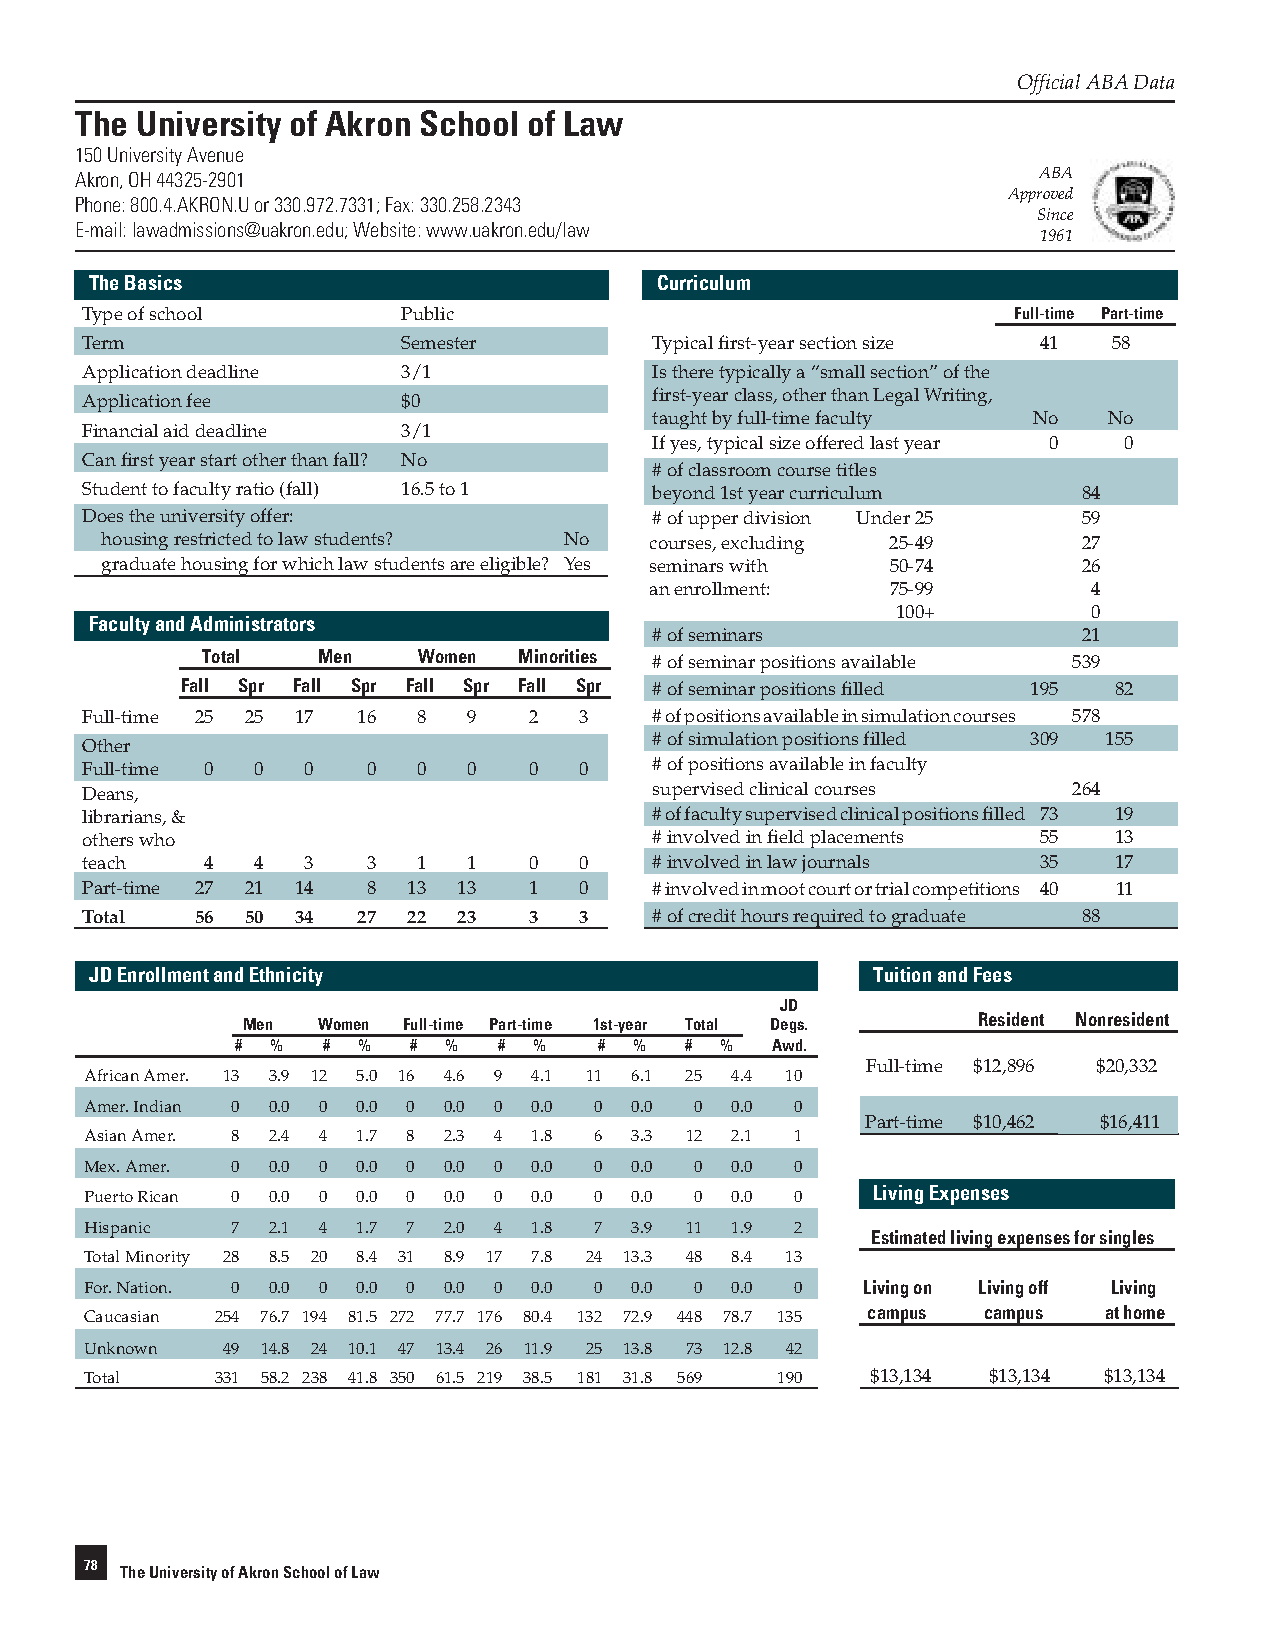
\includepdf[pages={1-2},nup=1x2,landscape=True]{Supplemental/abalsac_pre10.pdf}
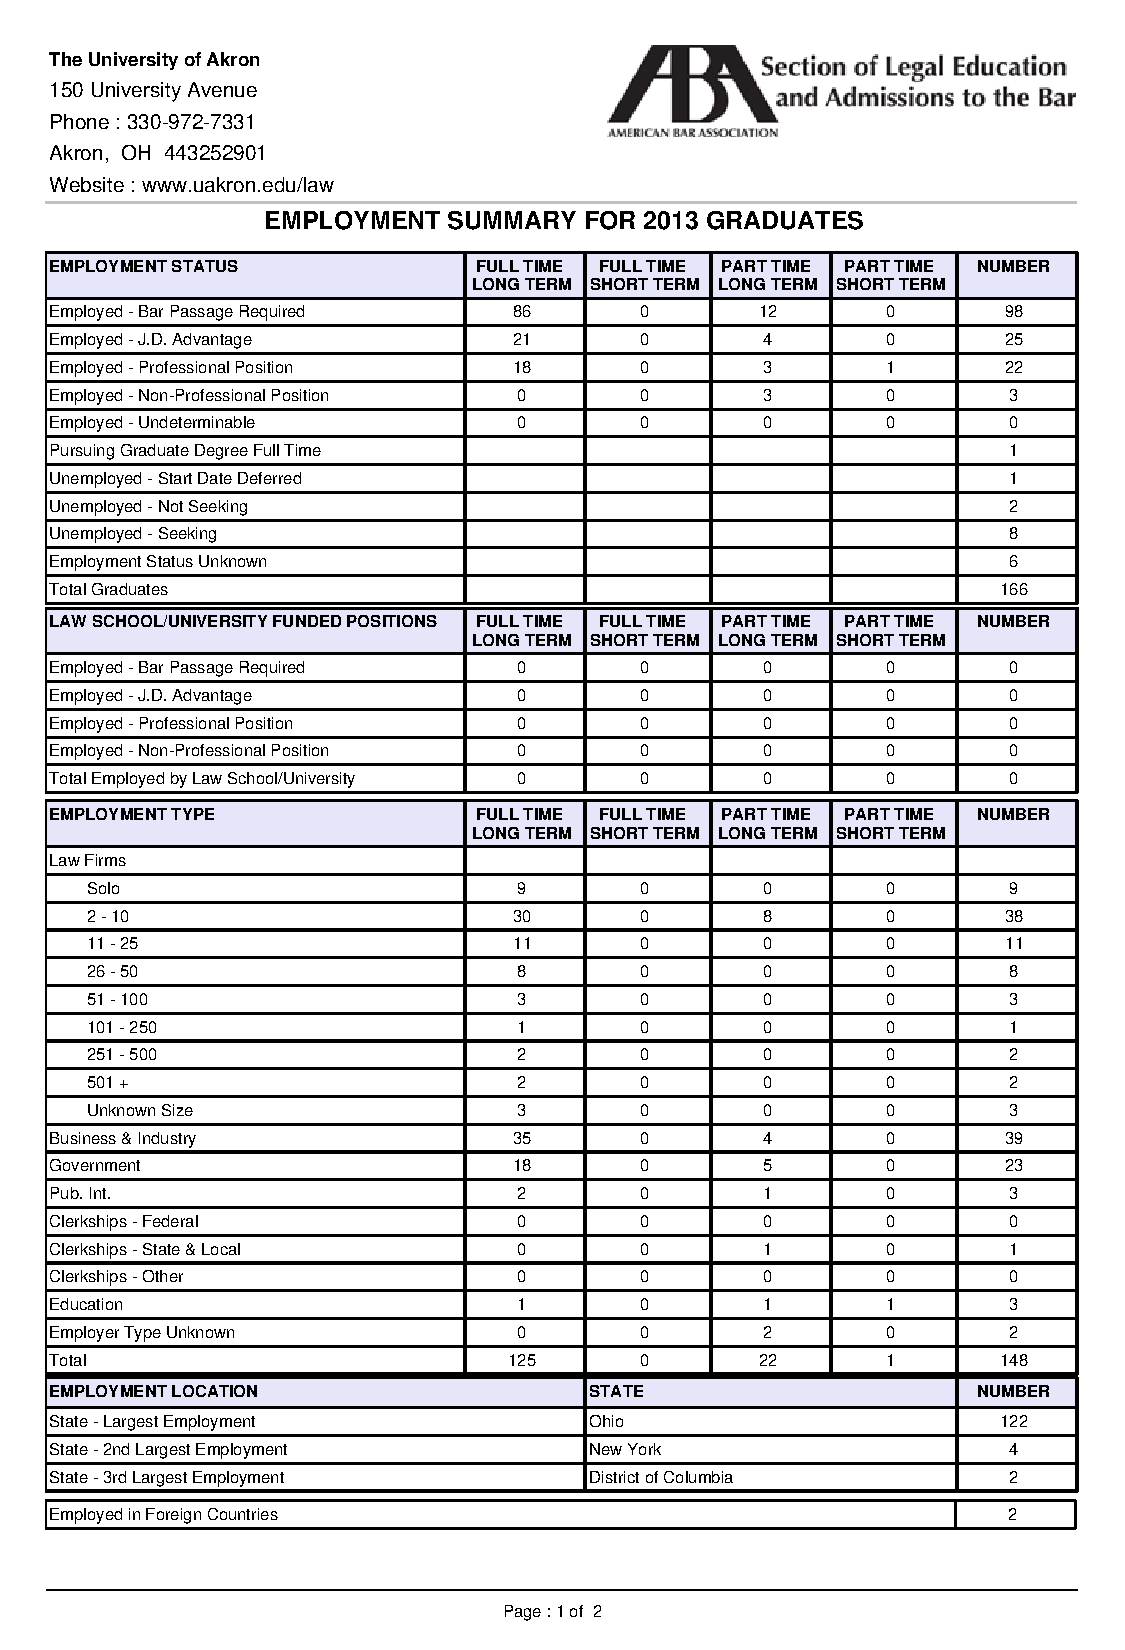
\includepdf[pages={1-2},nup=1x2,landscape=True]{Supplemental/abalsac_post10.pdf}


\section{Estimation Details}
This section gives specific details with regard to the estimators used in this paper. The first is for the application of the BBL estimator. The second gives a detailed description of the stage game simulation process.

\subsection{The BBL Estimator}
\label{app:bbl_estimator}
As in BBL, the value function for an active firm remaining in the market is constructed as

\begin{equation}
	V_j((R, g); \sigma, I, \theta) = \mathbb{E}\left[\sum_{t=0}^{\infty}\beta^t\Psi_j(\sigma, (R_t, g_t), \varepsilon_t|(R_0, g_0) = (R, g))\right]\cdot \theta = {\bf W}_j((R, g); \sigma)\cdot \tilde{\theta}
\label{eq:val_remaining}
\end{equation}
with the basis functions taking the form
\[
	\Psi_j = [\tilde{\pi}_j, r_j, r_j^2]'
\]
and $\tilde{\theta}\equiv[1, \delta_1, \delta_2]$. By linearity, $W_j$ can be simulated up to structural paraters $\tilde{\theta}$. The structural coefficients for the donation function can be estimated as usual with the BBL estimator based on Equation~\eqref{eq:val_remaining}.

Denoting an off-equilibrium policy $\tilde{\sigma}_j$, the equilibrium definition gives the condition
\begin{equation}
  W_j((R, g); \sigma_j^*, \sigma_{-j}^*)\cdot\tilde{\theta} \geq
  W_j((R, g); \tilde{\sigma}_j, \sigma_{-j}^*)\cdot\tilde{\theta}
  \label{eq:eqbm_condition}
\end{equation}
for all off-equilibrium policies. For the current application, I use a standard-normal additive perturbation to the estimates of school policy functions outlined in Section~\ref{sec:tuition_strategy}.

Following BBL, Equation~\eqref{eq:eqbm_condition} can be rewritten as
\begin{equation}
  m(\tilde{\sigma}_j; \tilde{\theta}) = [
    W_j((R, g); \sigma_j^*, \sigma_{-j}^*) -
    W_j((R, g); \tilde{\sigma}_j, \sigma_{-j}^*)
  ]\cdot\tilde{\theta}.
\end{equation}
The desired m-estimator can now be written as
\begin{equation}
  \min_{\tilde{\theta}}Q_n(\tilde{\theta}) = \frac{1}{K}\sum_{k=1}^K
    1(m(\tilde{\sigma}_{j, k}; \tilde{\theta}) > 0)
    m(\tilde{\sigma}_{j, k}; \tilde{\theta})^2,
\end{equation}
thus searching for parameter values that minimize profitable deviations from the optimal policy.

To estimate the distribution of entrance costs and scrap values, I exploit the fact that there has been no observed exit in this market to simulate an approximate value function with no exit included in the simulation. I further utilize Assumption~\ref{as:scrap} and Equation~\eqref{eq:entryscrap} to construct the equation
\begin{align}
  \Pr(\phi_i \leq V(\underline{r}, \underline{s})) &= 0.999 \notag \\
  \Rightarrow \Phi(V(\underline{r}, \underline{s}); \mu_\phi, \sigma^2_\kappa) &= 0.999 \label{eq:exit_moment}
\end{align}
The rest of the parameters can be estimated as follows
\begin{enumerate}
  \item Use approximate value function and predicted entrances to estimate entrance costs
  \item Use the moment equality from Equation~\eqref{eq:exit_moment} and, replacing $\sigma^2_\kappa$ with $\hat{\sigma}^2_\kappa$ from Step~1, estimate $\mu_\phi$ with the Method of Simulated Moments
  \item Update the approximate value function based on Step 2
  \item Iterate until $|\hat{\mu}_{\phi, \tau+1} - \hat{\mu}_{\phi, \tau}| < \epsilon$
\end{enumerate}

with $\tau$ the iteration count. I then estimate the distribution of entrance costs using predicted probabilities of entrance based on first-stage BBL estimates. 


\subsection{Stage Game Outcome Simulation Subroutine}
\label{app:appadmit_sim}

The required task is to simulate the outcomes of the application-admission stage game for a representative population of applicants and schools. The final goal of the simulation is to produce the function $f_{treat=0, 1}(outcome | Rank, Tuition)$, with $f$ a boosted random forest defined for either the period before ($treat=0$) or after ($treat=1$) the information regime chance and $outcome$ one of three variables: 1) median LSAT scores of matriculants, 2) median undergraduate GPA of matriculants, and 3) total number of matriculants.

The outcome functions are simulated for a given year $y$ in the set of possible years defined by $treat$ as follows:
\begin{enumerate}
  \item Draw $\hat{n}$ applicants with replacement from all reported applicants in $y$
  \item Select $n\times J$ data points $(OverallRank_j, Tuition_j, LSAT_i, GPA_i, treat, year)_{i\in n, j\in J}$ corresponding to each applicant/school combination to generate the simulation dataset
  \item For each 
  \item For each application, simulate admission based on predicted probability of a positive admission decision
  \item For each applicant with a non-zero number of admissions, simulate the decision to enroll at all based on the highest rank of admitting schools
  \item For each enrolling student, simulate the school to attend based on the highest predicted probability of attendance among the admitting schools
  \item Repeat $K$ times
\end{enumerate}
Each of the simulation runs results in an incoming class profile, consisting (among other things) of median LSAT and GPA scores and class size. Finally, average the results across the $K$ runs to get the dataset to which the $f$ can be fit, in this case with a gradient boosted regression tree.


%The details of the simulation are as follows. Having already obtained first-stage reduced form coefficients for the optimal policy function, I draw a set of 200 rank/state combinations from their joint empirical distribution. I also draw an initial wage level from the empirical marginal distribution for aggregate lawyer wages.

\section{Student Preferences}
\label{app:outside}
The preferences for students of any given observed quality must be calculated in order to determine total welfare effects of the information regime change. The next two sections outline identification and estimation of a student's utility for attending any given law school as well as her corresponding outside option.

\subsection{Identification of Student Utility}
\label{app:id_outside}
\begin{claim}
  Equation~\eqref{eq:student_welfare_ident} is sufficient to identify the value for student $i$ of attending school $j$.
\end{claim}
\begin{proof}
  Beginning with Equation~\eqref{eq:student_welfare_ident} and, for ease of notation, defining $\overline{u}_{ij} \equiv \overline{u}(A_i, R_j, I)$ and $f_{Mij} \equiv f_M(LSAT_i, GPA_i, R_j, t_j)$ and with $\tilde{\Phi}$ and $\tilde{\Phi}^{-1}$ denoting the normal distribution with variance $\sigma_u^2$ and quantile functions, respectively,
  \begin{align*}
    &&Pr(U_{ij}(t) > 0) &= f_{Mij} \\
    \Rightarrow&& Pr(\overline{u}_{ij} + \varepsilon_{ij} - t_j \geq 0) &= f_{Mij} \\
    \Rightarrow&& Pr(\varepsilon_{ij} \geq t_j - \overline{u}_{ij} ) &= f_{Mij} \\
    \Rightarrow&& \tilde{\Phi}(t_j - \overline{u}_{ij} ) &= f_{Mij} \\
    \Rightarrow&& (t_j - \overline{u}_{ij} ) &= \tilde{\Phi}^{-1}(f_{Mij}) \\
    \Rightarrow&& \overline{u}_{ij} &= t_j - \tilde{\Phi}^{-1}(f_{Mij})\\
  \end{align*}
  which implies identification given $\sigma_u^2$ since $f_{Mij}$ is non-parametrically identified in the data and $t_j$ is observed. Finally, $\sigma_u^2$ can be identified using variation within groups of applicants with the same application profile and best-choice school.
  % DOES THIS WORK WITH CONTINUOUS VARIABLES?
\end{proof}

\subsection{Estimation Details for Student Preferences}
\label{app:est_outside}
To compare estimates based on the two information regimes, I sample a population of students for each year $1, \dots, \overline{T}$, with $\overline{T}$ the cutoff year for forward simulation. Each student $i$ is drawn from the empirical distribution $\hat{F}(LSAT_i, GPA_i | treat)$, with the number of draws equal to the average number of applicants in a given year conditional on being in the treatment period or not. The size of the applicant pool is taken from the ABA-LSAC End-of-Year summary of law school applicants~\cite{abaeoy}.

To determine matriculation probability, I use estimates of admission and matriculation probabilities to first simulate the binary admission outcome for student $i$ (did admission happen?) and second, calculate the expected rank of a matriculating school $j$, should the student matriculate. I then estimate the tuition for school $j$ using the tuition policy function estimate. Finally, I use the estimates from the application-admission game to determine the probability of student $i$ matriculating to school $j$. This probability constitutes $f_{Mij}$.

\section{Tables and Figures}
\label{app:tables_figures}
\input{../Results/Initial/Tables/summary.tex}
\input{../Results/Initial/Tables/summary_appadmit.tex}
\input{../Results/Initial/Tables/summary_quant_GPA.tex}
\input{../Results/Initial/Tables/summary_quant_LSAT.tex}
\clearpage

\begin{figure}[htbp]
  \begin{center}
    \includegraphics{../Results/Initial/Figures/OverallRankAve.pdf}
    \caption{Evolution by Rank Quantile}
    \label{fig:rank_quantile}
  \end{center}
\end{figure}

\begin{figure}[htbp]
  \begin{center}
    \includegraphics{../Results/Initial/Figures/ratioAve.pdf}
    \caption{Evolution by Ratio Quantile}
    \label{fig:ratio_quantile}
  \end{center}
\end{figure}
\clearpage

\input{../Results/FirstStage/Tables/apps-rank.tex}
\input{../Results/FirstStage/Tables/apps-ratio.tex}
\input{../Results/FirstStage/Tables/sal25-rank.tex}
\input{../Results/FirstStage/Tables/sal25-ratio.tex}
\input{../Results/FirstStage/Tables/sal75-rank.tex}
\clearpage
\input{../Results/FirstStage/Tables/sal75-ratio.tex}
\input{../Results/FirstStage/Tables/tuition-rank.tex}
\input{../Results/FirstStage/Tables/tuition-ratio.tex}
\input{../Results/FirstStage/Tables/class-rank.tex}
\input{../Results/FirstStage/Tables/class-ratio.tex}
\input{../Results/FirstStage/Tables/lsat-rank.tex}
\clearpage
\input{../Results/FirstStage/Tables/lsat-ratio.tex}
\input{../Results/FirstStage/Tables/gpa-rank.tex}
\input{../Results/FirstStage/Tables/gpa-ratio.tex}
\clearpage
\newpage

\begin{figure}[htbp]
  \begin{center}
    \includegraphics{../Results/FirstStage/Figures/appadmit_importance.pdf}
    \caption{Application-Admission Game: Variable Importance}
    \label{fig:app_admit_importance}
  \end{center}  
\end{figure}

\begin{figure}[htbp]
  \begin{center}
    \includegraphics{../Results/FirstStage/Figures/appadmit_outcomes_treat0_importance.pdf}
    \caption{
      Application-Admission Outcome Functions (treat=0): Variable Importance
    }
    \label{fig:app_admit_outcome_0_importance}
  \end{center}  
\end{figure}

\begin{figure}[htbp]
  \begin{center}
    \includegraphics{../Results/FirstStage/Figures/appadmit_outcomes_treat1_importance.pdf}
    \caption{
      Application-Admission Outcome Functions (treat=1): Variable Importance
    }
    \label{fig:app_admit_outcome_1_importance}
  \end{center}  
\end{figure}

\begin{figure}[htbp]
  \begin{center}
    \includegraphics{../Results/FirstStage/Figures/fs_tuition_importance.pdf}
    \caption{Tuition Policy Function: Variable Importance}
    \label{fig:tuition_importance}
  \end{center}  
\end{figure}

\clearpage
\input{../Results/FirstStage/Tables/logitapp.tex}
\input{../Results/FirstStage/Tables/logitadmit.tex}
\input{../Results/FirstStage/Tables/logitmatric.tex}


\clearpage
\begin{figure}[htbp]
  \begin{center}
    \includegraphics{../Results/SecondStage/Figures/value_diff.pdf}
    \caption{Change in producer surplus function: $\Delta V(R)$}
    \label{fig:V_delta}
  \end{center}
\end{figure}

\begin{figure}[htbp]
\begin{center}
\includegraphics[width=\textwidth]{../Results/Secondstage/Figures/Dynamics/demandquantiles.pdf}
\caption{demandquantiles}
\label{fig:demandquantiles}
\end{center}
\end{figure}

\begin{figure}[htbp]
\begin{center}
\includegraphics[width=\textwidth]{../Results/Secondstage/Figures/Dynamics/MedianLSATquantiles.pdf}
\caption{MedianLSATquantiles}
\label{fig:MedianLSATquantiles}
\end{center}
\end{figure}

\begin{figure}[htbp]
\begin{center}
\includegraphics[width=\textwidth]{../Results/Secondstage/Figures/Dynamics/OverallRankquantiles.pdf}
\caption{OverallRankquantiles}
\label{fig:OverallRankquantiles}
\end{center}
\end{figure}

\begin{figure}[htbp]
\begin{center}
\includegraphics[width=\textwidth]{../Results/Secondstage/Figures/Dynamics/Tuitionquantiles.pdf}
\caption{Tuitionquantiles}
\label{fig:Tuitionquantiles}
\end{center}
\end{figure}

\begin{figure}[htbp]
\begin{center}
\includegraphics[width=\textwidth]{../Results/Secondstage/Figures/Dynamics/UndergraduatemedianGPAquantiles.pdf}
\caption{UndergraduatemedianGPAquantiles}
\label{fig:UndergraduatemedianGPAquantiles}
\end{center}
\end{figure}

%\begin{figure}[htbp]
%\begin{center}
%\includegraphics{../Results/Diagnostics/Dynamics/demandrank.pdf}
%\caption{demandrank}
%\label{fig:demandrank}
%\end{center}
%\end{figure}
%
%\begin{figure}[htbp]
%\begin{center}
%\includegraphics{../Results/Diagnostics/Dynamics/MedianLSATrank.pdf}
%\caption{MedianLSATrank}
%\label{fig:MedianLSATrank}
%\end{center}
%\end{figure}
%
%\begin{figure}[htbp]
%\begin{center}
%\includegraphics{../Results/Diagnostics/Dynamics/OverallRankrank.pdf}
%\caption{OverallRankrank}
%\label{fig:OverallRankrank}
%\end{center}
%\end{figure}
%
%\begin{figure}[htbp]
%\begin{center}
%\includegraphics{../Results/Diagnostics/Dynamics/Tuitionrank.pdf}
%\caption{Tuitionrank}
%\label{fig:Tuitionrank}
%\end{center}
%\end{figure}
%
%\begin{figure}[htbp]
%\begin{center}
%\includegraphics{../Results/Diagnostics/Dynamics/UndergraduatemedianGPArank.pdf}
%\caption{UndergraduatemedianGPArank}
%\label{fig:UndergraduatemedianGPArank}
%\end{center}
%\end{figure}
%
%\clearpage
%\begin{figure}[htbp]
%  \begin{center}
%    \includegraphics{../Results/SecondStage/Figures/value.pdf}
%    \caption{Value Functions}
%    \label{fig:value_functions}
%  \end{center}
%\end{figure}

%%%%%%%%%%%%%%%%%%%%%%
%%    REFERENCES    %%
%%%%%%%%%%%%%%%%%%%%%%
\clearpage
\bibliography{LawStructuralBib.bib}{}
\bibliographystyle{jpe}

\end{document}